% ============================================================
\chapter{Dünya Yerçekimi Modeli}
\label{ch:earth_model}
% ============================================================

Bir önceki bölümde, Legendre polinomları ve ilişkili Legendre fonksiyonlarının (Laplace denkleminin küresel koordinatlarda ayrılmasıyla) nasıl ortaya çıktığı, özdeğerlerin neden ayrıklaştığı ve bu yapıdan küresel harmonik bazın nasıl türetildiği ayrıntılı biçimde verildi. Bu bölümde aynı matematiksel çerçeve, \textbf{Dünya'nın gerçek} (küresel olmayan) yerçekimi alanını modellemek için yeniden ele alınacaktır.

\medskip
\noindent
Hedef; ideal iki-cisim yaklaşımındaki
\begin{equation}
U_0(r)=-\frac{\mu}{r},\qquad \mu\equiv GM
\label{eq:U0_def}
\end{equation}

potansiyelinden başlayarak,
Dünya'nın basıklığı ve kütle düzensizliklerinin (zonal/tesseral/sectoral bileşenler)
küresel harmonik katsayıları üzerinden nasıl taşındığını netleştirmektir. Bu sayede, $J_2$ başta olmak üzere $\bar C_{\ell,m},\bar S_{\ell,m}$ katsayılarının fiziksel yorumu ve sayısal propagasyondaki rolü tek bir çatı altında toplanacaktır.



% ===================== Dünya Küre Değil ====================
\newpage
\section{Dünya Küre Değil}
\label{sec:earth_not_perfect}

Merkezi (noktasal kütle) yaklaşımında potansiyel \eqref{eq:U0_def} yalnızca uzaklığa, yani $r$’ye bağlıdır.
Bu sonuç Newton’un küre teoremine dayanır ve ancak homojen, mükemmel küresel bir kütle dağılımı için geçerlidir.
Oysa Dünya bu ideal varsayımlardan belirgin biçimde sapar.
Kutuplarda basık ve ekvatorda şişkindir; iç yapısında yoğunluk dağılımı homojen değildir; topoğrafya ile okyanus--kıta farkları ve bölgesel jeolojik yapılar da yerel kütle anomalileri oluşturur \cite{Pavlis2008}.

\medskip
Bu sapmaların yerçekimi alanında bıraktığı iz \autoref{fig:grace_potato}'da görülür.
Şekildeki “patates” benzeri biçim Dünya’nın gerçek geometrisini değil, yerçekimi alanındaki uzaysal değişimleri abartarak görünür kılan bir temsili anlatır.
Renkler ve yüzeydeki kabarma ile çökme bölgeleri, potansiyelin yalnızca yarıçapa göre değil, Dünya üzerindeki konuma göre de değiştiğini net biçimde gösterir.

\begin{figure}[h]
    \centering
    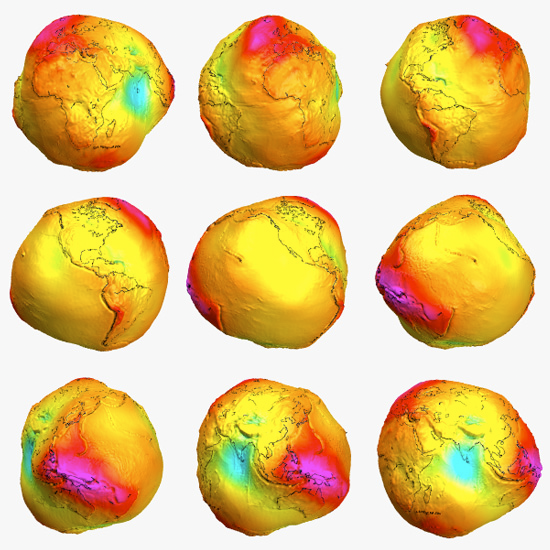
\includegraphics[width=0.9\linewidth]{Resimler/Dünya Modeli/GRACE Potato Model.png}
    \caption{GRACE/GRACE-FO verilerinden türetilen Dünya yerçekimi anomali alanının abartılmış görselleştirmesi.
    Renkler ve yüzey sapmaları, potansiyelin enlem ve boylam boyunca değiştiğini vurgular. Kırmızı renk yüksek gravite alanlarını temsil ederken, mavi renkli bölgeler daha düşük bölgeleri temsil etmektedir.}
    \label{fig:grace_potato}
\end{figure}

\newpage
Bu nedenle gerçek çekim potansiyeli tek başına $r$’nin bir fonksiyonu değildir; enlem ve boylama da bağlıdır.
Başka bir deyişle potansiyel $U(r,\theta,\lambda)$ şeklinde konuma bağlı bir yapı kazanır.
Önceki bölümde elde edilen Legendre ve ilişkili Legendre polinomları bu noktada devreye girer.
Bu fonksiyonlar açısal bağımlılığı düzenli bir biçimde ayrıştırmaya yarar ve küresel harmonikler aracılığıyla potansiyelin enlem ve boylam yönündeki değişimini sistematik olarak ifade etmemizi sağlar.


% ===================== Harmonik Sınıflar =======================
\section{Harmonik Sınıfları}
\label{sec:norm_and_Jn}

Dünya'nın dış bölgesinde ($r>R_E$) kütle yoğunluğu yoktur ($\rho=0$) ve potansiyel
\begin{equation}
\nabla^2 U = 0
\label{eq:laplace_outside}
\end{equation}
Laplace denklemini sağlar.
Önceki bölümde Laplace denkleminin küresel koordinatlarda ayrılmasıyla
boylam yönünde periyodik Fourier modlarının ve enlem yönünde associated Legendre fonksiyonlarının elde edildiği gösterilmişti.
Bu nedenle Dünya için ``doğal'' potansiyel yazımı, küresel harmonik baz üzerinde katsayılandırılmış bir açılımdır; potansiyel
\begin{equation}
U(r,\phi,\lambda)
=
-\frac{\mu}{r}
\left[
1
+
\sum_{\ell=2}^{\infty}
\left(\frac{R_E}{r}\right)^{\ell}
\sum_{m=0}^{\ell}
\overline{P}_{\ell}^{\,m}[\sin\phi]
\left(
\overline{C}_{\ell m}\cos m\lambda
+
\overline{S}_{\ell m}\sin m\lambda
\right)
\right]
\label{eq:earth_potential1}
\end{equation}
\noindent
şeklinde yazılır. Bu denklem, Dünya’nın kütle dağılımındaki düzensizlikleri küresel harmonikler cinsinden ifade eder.

Bu açılımı daha kompakt bir notasyonla ifade etmek için küresel harmonik baz fonksiyonları genellikle $Y_{\ell}^{m}$ ile gösterilir.
Burada $\overline{P}_{\ell}^{\,m}(\sin\phi)$ enlem bağımlılığını, $\cos(m\lambda)$ ve $\sin(m\lambda)$ terimleri ise boylam bağımlılığını taşır.
Gerçek (cos/sin) gösterimde modlar
\[
Y_{\ell, m}^{c}(\phi,\lambda)=\overline{P}_{\ell}^{\,m}[\sin\phi]\cos(m\lambda),
\qquad
Y_{\ell, m}^{s}(\phi,\lambda)=\overline{P}_{\ell}^{\,m}[\sin\phi]\sin(m\lambda)
\]
şeklinde yazılır ve \eqref{eq:earth_potential1} içindeki $\overline{C}_{\ell, m}$ ve $\overline{S}_{\ell, m}$ katsayıları bu modların ağırlıklarını belirler. Jeodezi literatürü ile tutarlılık açısından yaygın olan gerçek katsayılı (cos/sin) gösterim tercih edilmiştir.

\medskip
\noindent
Bu gösterimde $\ell$ (derece) ve $m$ (mertebe) indisleri, küre üzerindeki desenin hem \textbf{ölçeğini} hem de
\textbf{boylama bağlılığını} belirler: $\ell$ büyüdükçe temsil edilen yapılar daha küçük ölçekli hâle gelir;
$m$ ise terimin boylam $\lambda$ boyunca değişimini, yani boylam yönündeki Fourier modunu belirtir.
Bu nedenle küresel harmonikler, $m$’nin aldığı değerlere göre üç temel sınıfta incelenir:
\textbf{zonal} ($m=0$), \textbf{tesseral} ($0<m<\ell$) ve \textbf{sectoral} ($m=\ell$).
İzleyen alt bölümlerde bu sınıflar sırasıyla tanıtılacak; her birinin geometrik yorumu ve
Dünya yerçekimi alanındaki fiziksel karşılıkları incelenecektir.


\begin{center}
\setlength{\fboxsep}{6pt}
\setlength{\fboxrule}{0.6pt}
\fbox{%
\begin{minipage}{0.82\linewidth}
\textbf{Harmonik sınıfları (Zonal--Tesseral--Sectoral)}\\[4pt]
\begin{itemize}
    \item $\boldsymbol{m=0}\ \Rightarrow\ \text{boylamdan bağımsız bantlar (zonal)},$
    \item $\boldsymbol{m=\ell}\ \Rightarrow\ \text{boylam dilimleri (sectoral)},$
    \item $\boldsymbol{0<m<\ell}\ \Rightarrow\ \text{enlem--boylam ızgarası (tesseral)}.$
\end{itemize}
\end{minipage}%
}
\end{center}


% ------------------ Zonal Harmonikler -------------
\newpage
\subsection{Zonal Harmonikler ($m=0$)}
\label{subsec:zonal}

\textbf{Zonal} harmonikler $m=0$ koşuluyla tanımlanır; dolayısıyla \textbf{boylamdan bağımsızdır}
ve yalnızca enlem (veya kolatitüde) değişkenine bağlıdır.
Bu özellik, dönme ekseni etrafındaki eksenel simetriyi temsil eder.
Geometrik olarak zonal bileşenler, küre üzerinde \textbf{enlemlere paralel bantlar}
(kuşaklar) üretir: potansiyel (ve dolayısıyla yerçekimi) boylama göre değişmez, yalnızca enlemle değişir.

Zonal terimler çoğu zaman en baskın şekil sapmalarını taşır. Özellikle $\ell=2$ zonal terimi
(çoğu kaynakta $J_2$ ile ilişkilendirilir), Dünya’nın kutuplardan basık ve ekvatordan şişkin olmasını
(\emph{oblateness}) birinci mertebeden temsil eder. Daha yüksek dereceli zonal terimler ($\ell=3,4,\dots$),
bu genel şeklin üzerine daha ince ölçekli düzeltmeler ekleyerek bant yapısını giderek daha sık hâle getirir.

\begin{figure}[h]
    \centering
    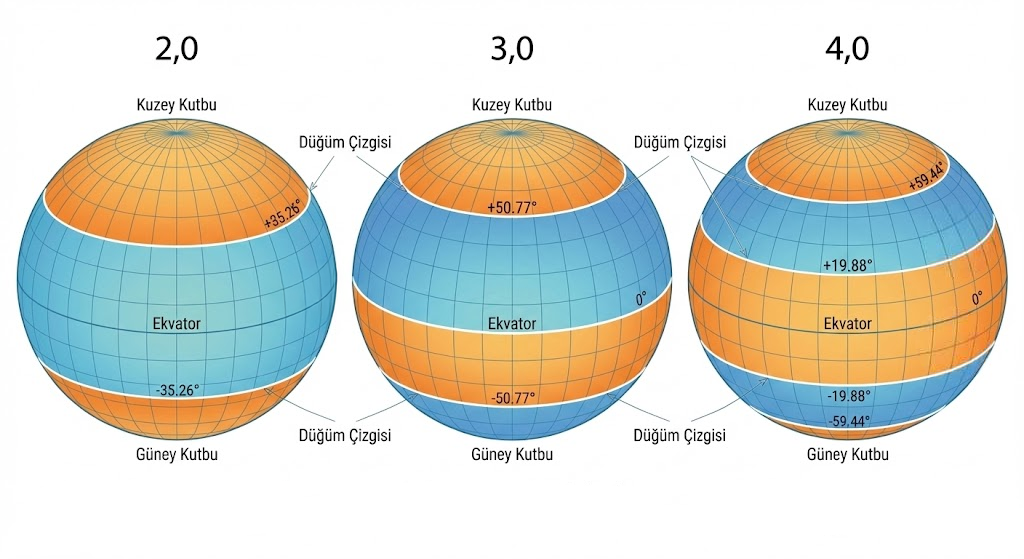
\includegraphics[width=1\linewidth]{Resimler/Dünya Modeli/Zonal Harmonikler.png}
    \caption{Zonal harmonikler ($m=0$) için $\ell=2,3,4$ örnekleri. Renkli bantlar (mavi pozitif, turuncu negatif) bölgeleri, bant sınırları ise düğüm dairelerini (nodal çizgileri) göstermektedir.}
    \label{fig:zonal_harmonics}
\end{figure}

\medskip
Şekil~\ref{fig:zonal_harmonics}’te görüldüğü üzere, zonal harmonikler için $m=0$ olduğundan
boylam bağımlılığı ortadan kalkar. Bu nedenle düğüm çizgileri \textbf{enlemlere paralel kapalı daireler} oluşturur.
Zonal bir harmonikte \textbf{$\ell$ adet düğüm dairesi} ve buna karşılık
\textbf{$\ell+1$ adet bant bölgesi} meydana gelir.


\subsubsection*{Düğüm enlemlerinin bulunması}

Zonal harmoniklerde ($m=0$) düğüm daireleri, açısal kısmın (enlem bağımlılığının) sıfır olduğu
enlemlere karşılık gelir. Bu nedenle düğüm enlemleri $\phi_i$, aşağıdaki koşuldan elde edilir:
\begin{equation}
P_\ell\!\bigl[\sin\phi_i\bigr]=0,
\qquad 
\phi_i\in\left(-\frac{\pi}{2},\frac{\pi}{2}\right).
\label{eq:zonal_nodes_phi}
\end{equation}
Burada $\phi$ jeosentrik enlemdir. Kökler $\phi=0$ (ekvator) etrafında simetriktir; bunun nedeni
Legendre polinomlarının parite özelliği $P_\ell[-x]=[-1]^\ell P_\ell(x)$’tir. Dolayısıyla bant yapısı
ekvatora göre düzenli bir simetri sergiler: $\ell$ tek ise ekvator bir düğümdür, $\ell$ çift ise
ekvator düğüm oluşturmaz.

\bigskip
\noindent
Düğüm enlemlerini bulmak için \eqref{eq:zonal_nodes_phi}’de $x=\sin\phi$ dönüşümü yapılır ve
$P_\ell(x)=0$ denkleminin kökleri hesaplanır. Küçük dereceler için bu kökler kapalı formda
açıkça gösterilebilir:

\begin{itemize}
\item \textbf{$\ell=2$:}
\[
P_2(x)=\tfrac{1}{2}(3x^2-1)
\quad\Rightarrow\quad
P_2(x)=0 \;\Rightarrow\; x=\pm \tfrac{1}{\sqrt{3}}.
\]
\[
\phi=\arcsin(x)=\pm \arcsin\!\left(\tfrac{1}{\sqrt{3}}\right)=\pm 35.26^\circ.
\]

\item \textbf{$\ell=3$:}
\[
P_3(x)=\tfrac{1}{2}(5x^3-3x)=\tfrac{1}{2}x(5x^2-3)
\quad\Rightarrow\quad
P_3(x)=0 \;\Rightarrow\; x=0,\ \pm\sqrt{\tfrac{3}{5}}.
\]
\[
\phi=\arcsin(x)=0^\circ,\qquad
\phi=\pm \arcsin\!\left(\sqrt{\tfrac{3}{5}}\right)=\pm 50.77^\circ.
\]

\item \textbf{$\ell=4$:}
\[
P_4(x)=\tfrac{1}{8}(35x^4-30x^2+3)
\quad\Rightarrow\quad
P_4(x)=0 \;\Rightarrow\; x=\pm 0.339981,\ \pm 0.861136.
\]
\[
\phi=\arcsin(x)
\quad\Rightarrow\quad
\phi\approx \pm 19.88^\circ,\ \pm 59.44^\circ.
\]

\end{itemize}

\begin{table}[h]
\centering
\caption{Zonal harmonikler için elde edilen düğüm enlemleri ($\phi_i$).}
\label{tab:zonal_nodes}
\renewcommand{\arraystretch}{1.25}
\begin{tabular}{@{} c c l @{}} 
\toprule
\textbf{Derece ($\ell$)} & \textbf{Düğüm Sayısı} & \textbf{Düğüm Enlemleri [deg]} \\
\midrule
2 & 2 & $\pm 35.26^\circ$ \\
3 & 3 & $0^\circ,\ \pm 50.77^\circ$ \\
4 & 4 & $\pm 19.88^\circ,\ \pm 59.44^\circ$ \\
\bottomrule
\end{tabular}
\end{table}



% --------------- Sectoral Harmonikler ----------------
\subsection{Sectoral Harmonikler ($m=\ell$)}
\label{subsec:sectoral}

\textbf{Sectoral} terimler $m=\ell$ koşuluyla tanımlanır.
Bu sınıfta hem enleme hem de boylama bağlılık en güçlü halini alır. Sectoral harmonikler küreyi boylam doğrultusunda ``dilimlere'' ayıran bir desen üretir: boylamda değişim maksimumdur ve desen, meridyenler boyunca sıkça tekrar eder.
$m$ (dolayısıyla $\ell$) arttıkça dilim sayısı artar; yani daha fazla sayıda, daha dar boylam bölgesi oluşur. Bu ``dilimlenme'' karakteri, farklı $\ell$ değerleri için örnek olarak
Şekil~\ref{fig:sectoral_harmonics}'te görülebilir.

\medskip
Fiziksel açıdan sectoral bileşenler,
tam eksen-simetrik olmayan ve belirli boylamlarda tekrarlayan kütle düzensizliklerini
temsil etmede etkilidir. Bu tür terimler, özellikle
tesseral/sectoral bileşenlerin baskın olduğu gezegenlerde veya bölgesel kütle anomalilerinde
yerçekimi alanına belirgin katkılar yapabilir.

\begin{figure}[h]
    \centering
    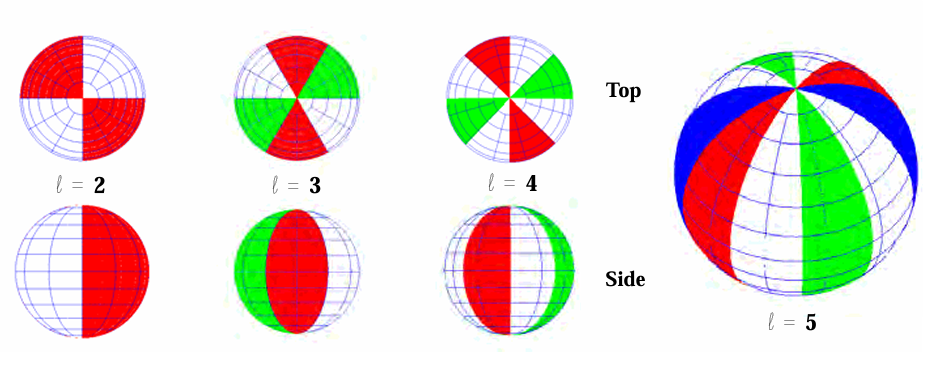
\includegraphics[width=1\linewidth]{Resimler/Dünya Modeli/Sectoral Harmonikler.png}
    \caption{Sectoral harmonikler ($m=\ell$) için örnek desenler: $\ell=2,3,4$ durumlarında üst (Top) ve yan (Side) görünüşler. Renkli bölgeler negatif, beyaz bölgeler ise pozitif katkıları göstermekte.}
    \label{fig:sectoral_harmonics}
\end{figure}


% ------------- Tesseral Harmonikler --------------

\subsection{Tesseral Harmonikler ($0<m<\ell$)}
\label{subsec:tesseral}

\textbf{Tesseral} terimler $0<m<\ell$ aralığıyla tanımlanır.
Bu sınıf, zonal ($m=0$) ile sectoral ($m=\ell$) arasında bir ``ara bölge'' gibidir: hem enleme hem de boylama bağlıdır, ancak sectoral kadar ``tam dilimli'' bir yapı vermez. Ortaya çıkan desen genellikle küre üzerinde bir \textbf{ızgara/karo} \emph{tessera}) görünümüne benzetilir; çünkü hem meridyen hem paralel yönünde işaret değişimleri (sıfır çizgileri) görülür.
Bu karo-benzeri desen karakteri, farklı $(\ell,m)$ çiftleri için örnek olarak Şekil~\ref{fig:tesseral_harmonics}'te gösterilmiştir.

\begin{figure}[h]
    \centering
    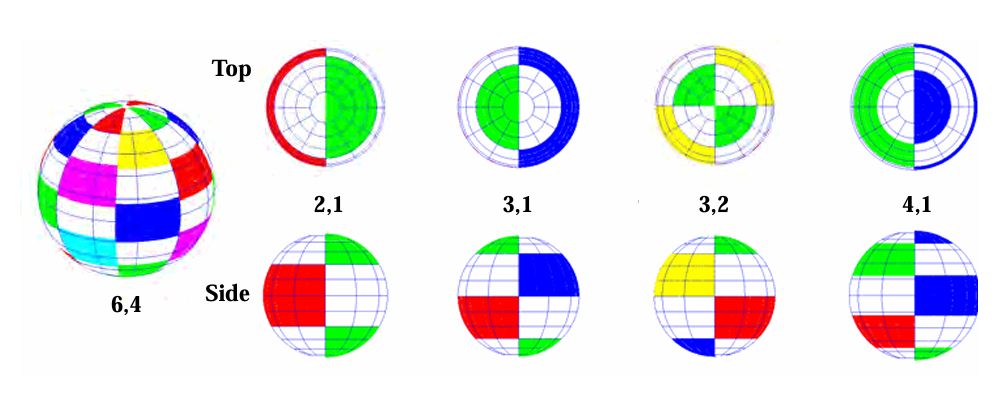
\includegraphics[width=1\linewidth]{Resimler/Dünya Modeli/Tesseral Harmonikler.png}
    \caption{Tesseral harmonikler ($0<m<\ell$) için örnek desenler: seçili $(\ell,m)$ çiftlerinde üst (Top) ve yan (Side) görünüşlerde oluşan ``karo'' (\emph{tessera}) benzeri işaret değişimleri. Renkli bölgeler negatif, beyaz bölgeler ise pozitif katkıları göstermekte.}
    \label{fig:tesseral_harmonics}
\end{figure}

Bazı kaynaklarda sectoral terimler, tesseral sınıfının
özel bir alt durumu gibi sunulabilir (çünkü $m=\ell$ de temelde boylama bağımlıdır). Ancak uygulamada, $m=\ell$ durumunun desen karakteri ve matematiksel davranışı (Şekil~\ref{fig:sectoral_harmonics}'teki belirgin ``dilimlenme'' gibi) daha ayırt edici olduğu için sectoral terimler çoğu zaman ayrı bir başlık altında incelenir.


% ================ J_l Terimlerinin Etkisi =============
\newpage
\section{\texorpdfstring{$J_\ell$}{J\_l} Terimleri ve Etkileri}

Zonal harmonikler ($m=0$) söz konusu olduğunda, literatürde iki farklı katsayı gösterimine sıklıkla rastlanır. Kullanım yaygınlığı nedeniyle $C_{\ell,0}$ katsayısı yerine genellikle $J_{\ell}$ notasyonu tercih edilmektedir. Ancak bu iki notasyon arasında bir işaret farkı bulunduğu unutulmamalıdır:

\begin{equation}
    C_{\ell,0} = - J_{\ell}
    \label{eq:C_J_relation}
\end{equation}

% ----------------- J_l ve C_bar arasındaki ilişki ---------
\subsection{\texorpdfstring{$J_\ell$ ile $\bar C_{\ell,0}$ İlişkisi}{J\_l ile C\_bar\_\{l,0\} İlişkisi}}
\label{subsec:Jn_relation}

Literatürde yerçekimi potansiyeli, klasik olarak \textbf{normalize edilmemiş} $J_{\ell}$ katsayıları kullanılarak şu formda ifade edilir:
\begin{equation}
U(r,\phi)
=
-\frac{\mu}{r}
\left[
1
+
\sum_{\ell=2}^{\infty}
J_\ell
\left(\frac{R_E}{r}\right)^\ell
P_\ell[\sin\phi]
\right].
\label{eq:zonal_potential}
\end{equation}
Burada $P_\ell[\sin\phi]$ yalnızca enleme bağlı Legendre polinomudur; dolayısıyla $m = 0$ olduğundan bileşenlerinde boylam etkisi yoktur. $J_\ell$ katsayısı, $\ell$ dereceli zonal harmonik katkının büyüklüğünü belirler. Özellikle $\ell=2$ için $J_2$, Dünya’nın basıklığını (\emph{oblateness}) temsil eden en baskın terimdir.

Ancak modern jeodezik modeller (örneğin EGM96, EGM2008), katsayı verilerini küresel harmonik bazının ortogonalliğini korumak amacıyla \textbf{tam-normalize} (\emph{fully normalized}) $\bar C_{\ell,0}$ formunda sunar. Bu iki gösterim fiziksel olarak eşdeğerdir; aralarındaki fark, normalizasyon tanımından kaynaklanan sabit bir ölçek çarpanıdır.

Jeodezide yaygın kullanılan dönüşüm şöyledir:
\begin{equation}
J_\ell = -\sqrt{2\ell+1}\,\bar C_{\ell,0},
\qquad \bar S_{\ell,0}=0
\label{eq:Jn_Cn0_relation}
\end{equation}
Bu ifadede $\sqrt{2\ell+1}$ çarpanı \textbf{normalizasyon farkını} temsil eder. $m=0$ (zonal) terimler için sinüs katsayısı bulunmadığından $\bar S_{\ell,0}=0$ olarak belirtilir.

Örneğin en sık kullanılan $\ell=2$ terimi için bu ilişki
\begin{equation}
J_2 = -\sqrt{5}\,\bar C_{2,0}
\label{eq:J2_C20}
\end{equation}
haline gelir. Dolayısıyla bir yerçekimi modelinden veri alınırken, katsayıların \textbf{normalize mi yoksa normalize edilmemiş mi} olduğuna ve kullanılan işaret konvansiyonuna mutlaka dikkat edilmelidir. Aksi halde, aynı fiziksel büyüklük farklı sayısal değerlerle ifade edileceğinden analizlerde ölçek hataları oluşabilir.

% ------------------ Oblateness ------------------
\newpage
\subsection{$J_2$: Basıklık (Oblateness)}
\label{subsec:J2_physical}

Zonal terimler içinde pratikte en baskın olanı $J_2$’dir.
Bunun temel nedeni, Dünya’nın küreden sapmasının en büyük bileşeninin
ekvator şişkinliği (kutuplardan basıklık) olmasıdır.
Basıklık (\emph{oblateness}) şu şekilde tanımlanır:
\begin{equation}
    oblateness = \frac{R_{ekvator} - R_{kutup}}{R_{ekvator}}
    \label{eq:oblateness}
\end{equation}
Dünya için yaklaşık $R_{ekvator} \approx 6378\,\mathrm{km}$ ve $R_{kutup} \approx 6357\,\mathrm{km}$ alındığında
\[
oblateness \approx \frac{6378-6357}{6378} \approx 3.29\times 10^{-3}
\]
bulunur (daha hassas yarıçap değerleriyle bu oran $\sim 3.35\times 10^{-3}$ mertebesindedir).

Burada önemli nokta şudur: \eqref{eq:oblateness} \textbf{geometrik} bir ölçüdür; $J_2$ ise Dünya’nın kütle dağılımının
\textbf{ikinci derece zonal} bileşenini (gravitasyonel ``quadrupole'') temsil eder.
İkisi birebir aynı nicelik değildir; ancak Dünya’daki ekvator şişkinliği hem şekli hem de kütle dağılımını belirgin biçimde
küresel simetriden saptırdığı için, pratikte en baskın zonal katsayının $J_2$ olması beklenir.

\eqref{eq:zonal_potential} içinde yalnızca $\ell=2$ terimini tutup
$P_2[x]=\tfrac12(3x^2-1)$ ve $x=\sin\phi$ yazarsak,
$J_2$’nin potansiyele katkısı enleme bağlı, ``bant'' yapılı bir düzeltme olarak görülür:
ekvator civarında ve kutuplara yakın bölgelerde potansiyel/ivme dağılımı farklılaşır.
Bu tür bir fark, her turda tekrar tekrar etki ettiği için yörünge elemanlarında \textbf{birikimli} (seküler) değişimlere yol açabilir.
Bu nedenle $J_2$, iki-cisim yaklaşımına eklenen \textbf{ilk düzeltme} katsayısı olarak çoğu yörünge probleminde ayrıcalıklı bir yere sahiptir.

Tipik büyüklük olarak
\[
J_2 \approx 1.08263\times10^{-3}
\]
mertebesindedir (seçilen yerçekimi modeli ve işaret/normalizasyon konvansiyonuna bağlı küçük farklar olabilir).
Bu değer, $J_2$’nin neden çoğu uygulamada ``ilk düzeltme'' olarak ele alındığını açıklar:
$J_2$ ihmal edildiğinde, özellikle LEO’da $\Omega$ ve $\omega$ sürüklenmeleri kısa sürede büyük hatalara dönüşür.


% ============================================================
% 2.1 -- 2.3 : J2 etkisi için ortak kurulum + GVE/LPE ile türetim
% ============================================================

\subsection*{RTN Ayrışımı}
\label{subsec:J2_setup}

Dünya’nın (yaklaşık) eksenel simetrik basıklığını temsil eden $J_2$ teriminin yörünge elemanlarına etkisini iki farklı formalizmle elde edebiliriz:
(i) Gauss Değişim Denklemleri (GVE) ve
(ii) Lagrange Gezegen Denklemleri (LPE).
Her iki yaklaşım da aynı fiziksel sonucu verir; fark, birinin doğrudan \textbf{ivme} (kuvvet) bileşenleri üzerinden, diğerinin ise \textbf{bozucu potansiyel} üzerinden ilerlemesidir.

\paragraph{Kepler elemanları ve yardımcı büyüklükler.}
Klasik yörünge (\emph{osculating}) elemanları
\[
(a,\;e,\;i,\;\Omega,\;\omega,\;M)
\]
kullanıyoruz. Gerçek anomali (\emph{True Anomaly}) $f$ için , enlem argümanı (\emph{argument of latitude}):
\[
u \;\triangleq\; \omega + f
\]
olarak tanımlıdır. Yarı parametre (\emph{semi-latus rectum})
\[
p \;\triangleq\; a(1-e^2),\qquad
r \;=\; \frac{p}{1+e\cos f}.
\]
Özgül açısal momentum büyüklüğü
\[
h \;\triangleq\; \|\mathbf r\times \mathbf v\| \;=\; \sqrt{\mu p},
\]
ve ortalama hareket
\[
n \;\triangleq\; \sqrt{\frac{\mu}{a^3}}
\]
şeklindedir. Burada $\mu=GM$ Dünya’nın çekim parametresidir.

\paragraph{RTN (Radial--Transverse--Normal) çerçevesi.}
Konum vektörü $\mathbf r$ ve hız vektörü $\mathbf v$ ile
\[
\hat{\mathbf R} \triangleq \frac{\mathbf r}{r},\qquad
\hat{\mathbf N} \triangleq \frac{\mathbf h}{h},\qquad
\hat{\mathbf T} \triangleq \hat{\mathbf N}\times \hat{\mathbf R}
\]
birim vektörleri tanımlanır.
Herhangi bir bozucu ivme $\mathbf a_p$ RTN bileşenlerine ayrıştırılır:
\[
a_R \triangleq \mathbf a_p\cdot \hat{\mathbf R},\qquad
a_T \triangleq \mathbf a_p\cdot \hat{\mathbf T},\qquad
a_N \triangleq \mathbf a_p\cdot \hat{\mathbf N},
\]
dolayısıyla
\[
\mathbf a_p \;=\; a_R\hat{\mathbf R} + a_T\hat{\mathbf T} + a_N\hat{\mathbf N}.
\]

\paragraph{$J_2$ potansiyeli ve bozucu fonksiyon.}
Dünya’nın eksenel simetrik (zonal) $J_2$ düzeltmesi ile,
yerçekimi potansiyelini (birim kütle başına) şu şekilde yazıyoruz:

\begin{equation}
U(r,\phi) \;=\; -\frac{\mu}{r}\Bigg[1 - J_2\Big(\frac{R_E}{r}\Big)^2 P_2[\sin\phi]\Bigg],
\qquad
P_2[x]=\frac{1}{2}(3x^2-1),
\label{eq:U_J2_def}
\end{equation}

burada $R_E$ ekvator yarıçapı ve $\phi$ jeosantrik enlemdir.
Merkezi ($-\mu/r$) terimi ayırırsak, $J_2$’ye karşılık gelen \textbf{bozucu potansiyel}
\[
\mathcal R_{J_2} \;\triangleq\; U + \frac{\mu}{r}
\;=\; \frac{\mu R_E^2 J_2}{2r^3}\,(3\sin^2\phi - 1)
\]
olur. Eksenel simetri nedeniyle $\phi$’yi yörünge elemanlarıyla bağlamak için
\[
z = r\sin\phi,\qquad
z = r\sin i \sin u
\;\;\;\Rightarrow\;\;\;
\sin\phi = \sin i \sin u
\]
kullanacağız.

\paragraph{$J_2$ ivmesinin RTN bileşenleri.}
$J_2$ etkisini GVE’de kullanmak için $\mathbf a_{J_2} = -\nabla \mathcal R_{J_2}$
ivmesini RTN’ye projekte ederiz. Standart sonuçlar şu biçimdedir:
\begin{subequations}\label{eq:J2_RTN_acc}
\begin{align}
a_R \;&=\; -\frac{3}{2}\,J_2\,\frac{\mu R_E^2}{r^4}\Big(1 - 3\sin^2 i\,\sin^2 u\Big), \label{eq:aR_J2}\\
a_T \;&=\; -3\,J_2\,\frac{\mu R_E^2}{r^4}\,\sin^2 i\,\sin u\,\cos u, \label{eq:aT_J2}\\
a_N \;&=\; -3\,J_2\,\frac{\mu R_E^2}{r^4}\,\sin i\,\cos i\,\sin u. \label{eq:aN_J2}
\end{align}
\end{subequations}
Bu üç bileşen, GVE veya Cowell propagasyonunda doğrudan kullanılabilir.

\paragraph{Yörünge ortalaması (seküler terimler).}
Özel yörüngeler (Sun-synchronous, kritik eğim/Molniya vb.) çoğunlukla seküler (uzun dönemli) oranlara dayanır. Bu yüzden, bir periyot boyunca \textbf{yörünge ortalaması} operatörünü tanımlıyoruz:
\begin{equation}
\big\langle (\cdot)\big\rangle \;\triangleq\;
\frac{1}{2\pi}\int_0^{2\pi} (\cdot)\, dM
\;=\;\frac{1}{2\pi}\int_0^{2\pi} (\cdot)\,\frac{r^2}{a^2\sqrt{1-e^2}}\,df.
\label{eq:orbit_average}
\end{equation}
Bu ortalamada kısa-periyotlu (periyot içinde salınan) terimler sıfıra gider, seküler drift oranları kalır.

% ------------------------------------------------------------
\subsection{Gauss Değişim Denklemleri (GVE)}
\label{subsec:J2_GVE}

GVE, bozucu ivmenin RTN bileşenleri cinsinden yörünge eleman türevlerini verir. Özellikle $\dot\Omega$ ve
$\dot\omega$ seküler oranları kritik olduğu için, önce ilgili GVE formüllerini yazıyoruz (klasik elemanlar için):

{%
\setlength{\fboxsep}{6pt}% kutu iç boşluğu
\setlength{\fboxrule}{0.6pt}% kutu çizgi kalınlığı
\begin{center}
\fbox{%
\begin{minipage}{0.97\linewidth}
\begin{subequations}\label{eq:GVE_basic}
\begin{align}
\dot a \;&=\; \frac{2a^2}{h}\Big[e\sin f\,a_R + \frac{p}{r}a_T\Big], \label{eq:GVE_a}\\[3pt]
\dot e \;&=\; \frac{1}{h}\Big[p\sin f\,a_R + \big((p+r)\cos f + re\big)a_T\Big], \label{eq:GVE_e}\\[3pt]
\dot i \;&=\; \frac{r\cos u}{h}\,a_N, \label{eq:GVE_i}\\[3pt]
\dot\Omega \;&=\; \frac{r\sin u}{h\sin i}\,a_N, \label{eq:GVE_Om}\\[3pt]
\dot\omega \;&=\; \frac{1}{he}\Big[-p\cos f\,a_R + (p+r)\sin f\,a_T\Big]
\;-\;\frac{r\sin u}{h}\cot i\,a_N, \label{eq:GVE_om}\\[3pt]
\dot f \;&=\; \frac{h}{r^2} + \frac{1}{he}\Big(p\cos f\,a_R - (p+r)\sin f\,a_T\Big). \label{eq:gauss_f}
\end{align}
\end{subequations}
\end{minipage}%
}%
\end{center}
}%

Burada $u=\omega+f$ ve $p=a(1-e^2)$’dir.



\subsubsection*{(i) Düğüm hattı dönümü: $\langle\dot\Omega\rangle$}

\eqref{eq:GVE_Om} içine $a_N$ bileşenini \eqref{eq:aN_J2} yerleştiriyoruz:
\[
\dot\Omega
\;=\;\frac{r\sin u}{h\sin i}\Bigg(-3J_2\frac{\mu R_E^2}{r^4}\sin i\cos i\,\sin u\Bigg)
\;=\; -\frac{3J_2\mu R_E^2}{h}\,\frac{\cos i}{r^3}\,\sin^2 u.
\]
Yörünge ortalaması alındığında,
$\sin^2 u = \tfrac12(1-\cos 2u)$ olduğundan $\cos 2u$ içeren terimler periyot boyunca
sıfıra gider ve
\[
\Big\langle \frac{\sin^2 u}{r^3}\Big\rangle
\;=\;\frac{1}{2}\Big\langle \frac{1}{r^3}\Big\rangle.
\]
Ayrıca bilinen sonuç
\[
\Big\langle \frac{1}{r^3}\Big\rangle
\;=\;\frac{1}{a^3(1-e^2)^{3/2}}
\]
kullanılır. Böylece
\begin{equation}
\boxed{
\big\langle \dot\Omega \big\rangle
\;=\; -\frac{3}{2}\,J_2\,n\Big(\frac{R_E}{p}\Big)^2\cos i
}
\label{eq:Omega_secular_J2}
\end{equation}
elde edilir.

\noindent
Bu bağıntı iki kritik yorumu doğrudan verir:
(i) seküler RAAN driftinin büyüklüğü $\cos i$ ile ölçeklenir; dolayısıyla eğim değiştikçe drift hızı değişir, (ii) $i=90^\circ$ (polar yörünge) için $\cos i=0$ olduğundan seküler RAAN drift sıfırlanır. Buna karşın, osculating (kısa-periyot) salınımlar tek tek yörüngeler üzerinde gözlenmeye devam eder.

\begin{figure}[h]
    \centering
    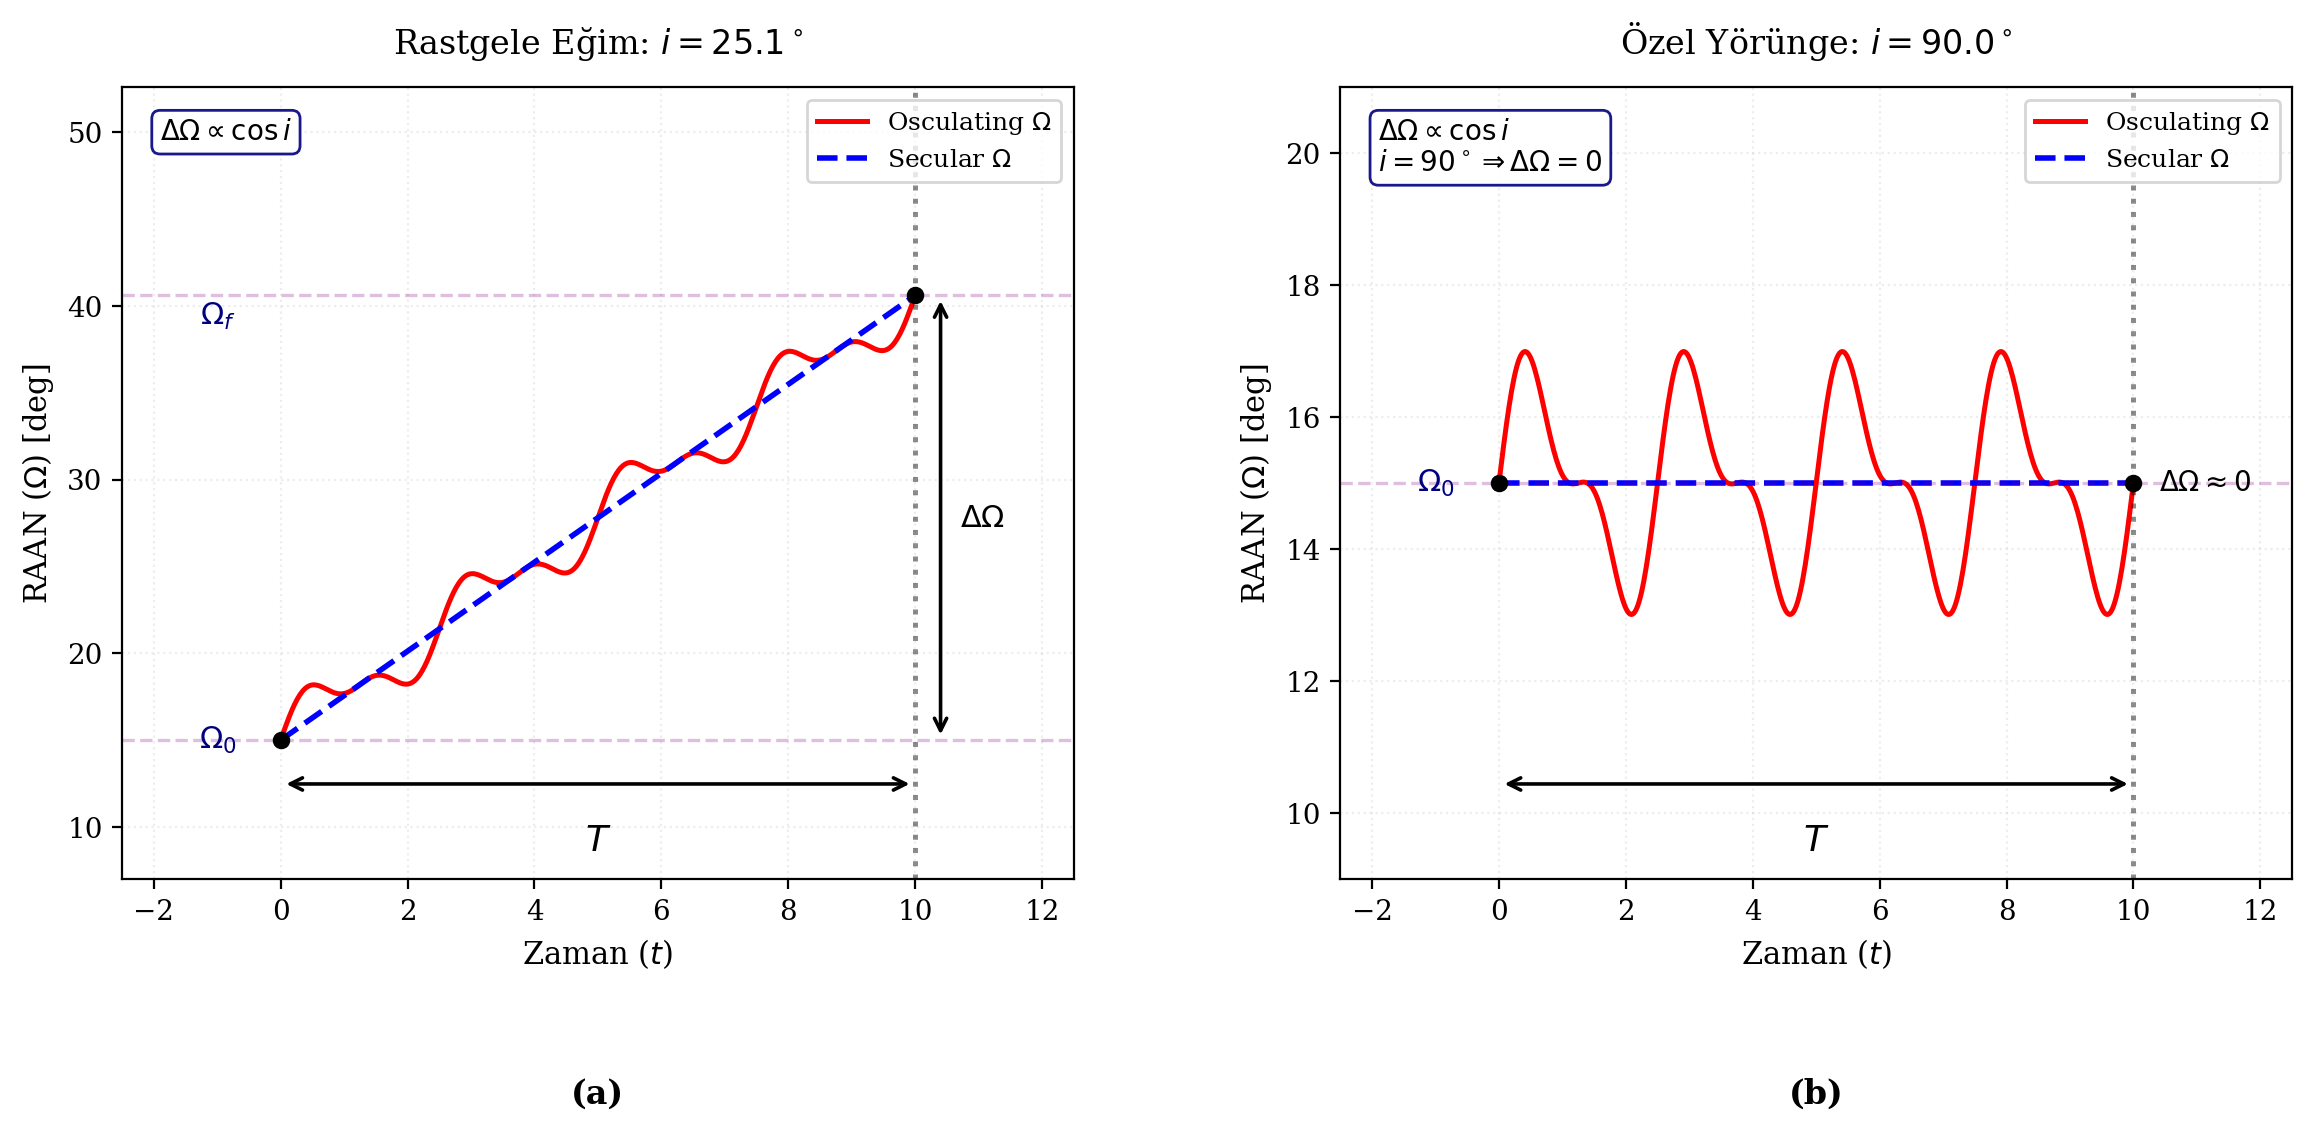
\includegraphics[width=1\linewidth]{Resimler/Dünya Modeli/RAAN Shift.png}
    \caption{J$_2$ etkisi altında RAAN ($\Omega$) değişimi: osculating (kırmızı) ve seküler/ortalama (mavi kesikli) bileşenlerin karşılaştırılması.
    (a) Genel bir eğiklikte $\Delta\Omega \neq 0$ olup seküler drift lineerdir.
    (b) Polar yörüngede ($i=90^\circ$) $\cos i = 0$ nedeniyle seküler drift yaklaşık sıfırdır; yalnızca kısa-periyot salınımlar kalır.}
    \label{fig:raan_shift_j2}
\end{figure}



\subsubsection*{(ii) Perigee dönümü: $\langle\dot\omega\rangle$}

\eqref{eq:GVE_om} ifadesine $a_R,a_T,a_N$ (bkz. \eqref{eq:J2_RTN_acc}) yerleştirilir.
Bu adımda $\sin u\cos u$ ve $\sin^2u$ gibi terimler oluşur. Periyot ortalamasında
$\sin 2u$ içeren terimler sıfıra gider; $\sin^2u$ ve $\cos^2u$ terimleri ise
$\tfrac12\langle 1/r^3\rangle$ şeklinde katkı verir.
Ayrıca $h=\sqrt{\mu p}$ ve $\langle 1/r^3\rangle$ kullanılarak sadeleştirilince,
seküler perigee dönüm oranı
\begin{equation}
\boxed{
\big\langle \dot\omega \big\rangle
\;=\; \frac{3}{4}\,J_2\,n\Big(\frac{R_E}{p}\Big)^2\big(5\cos^2 i - 1\big)
}
\label{eq:omega_secular_J2}
\end{equation}
olarak bulunur.

\begin{figure}[h]
    \centering
    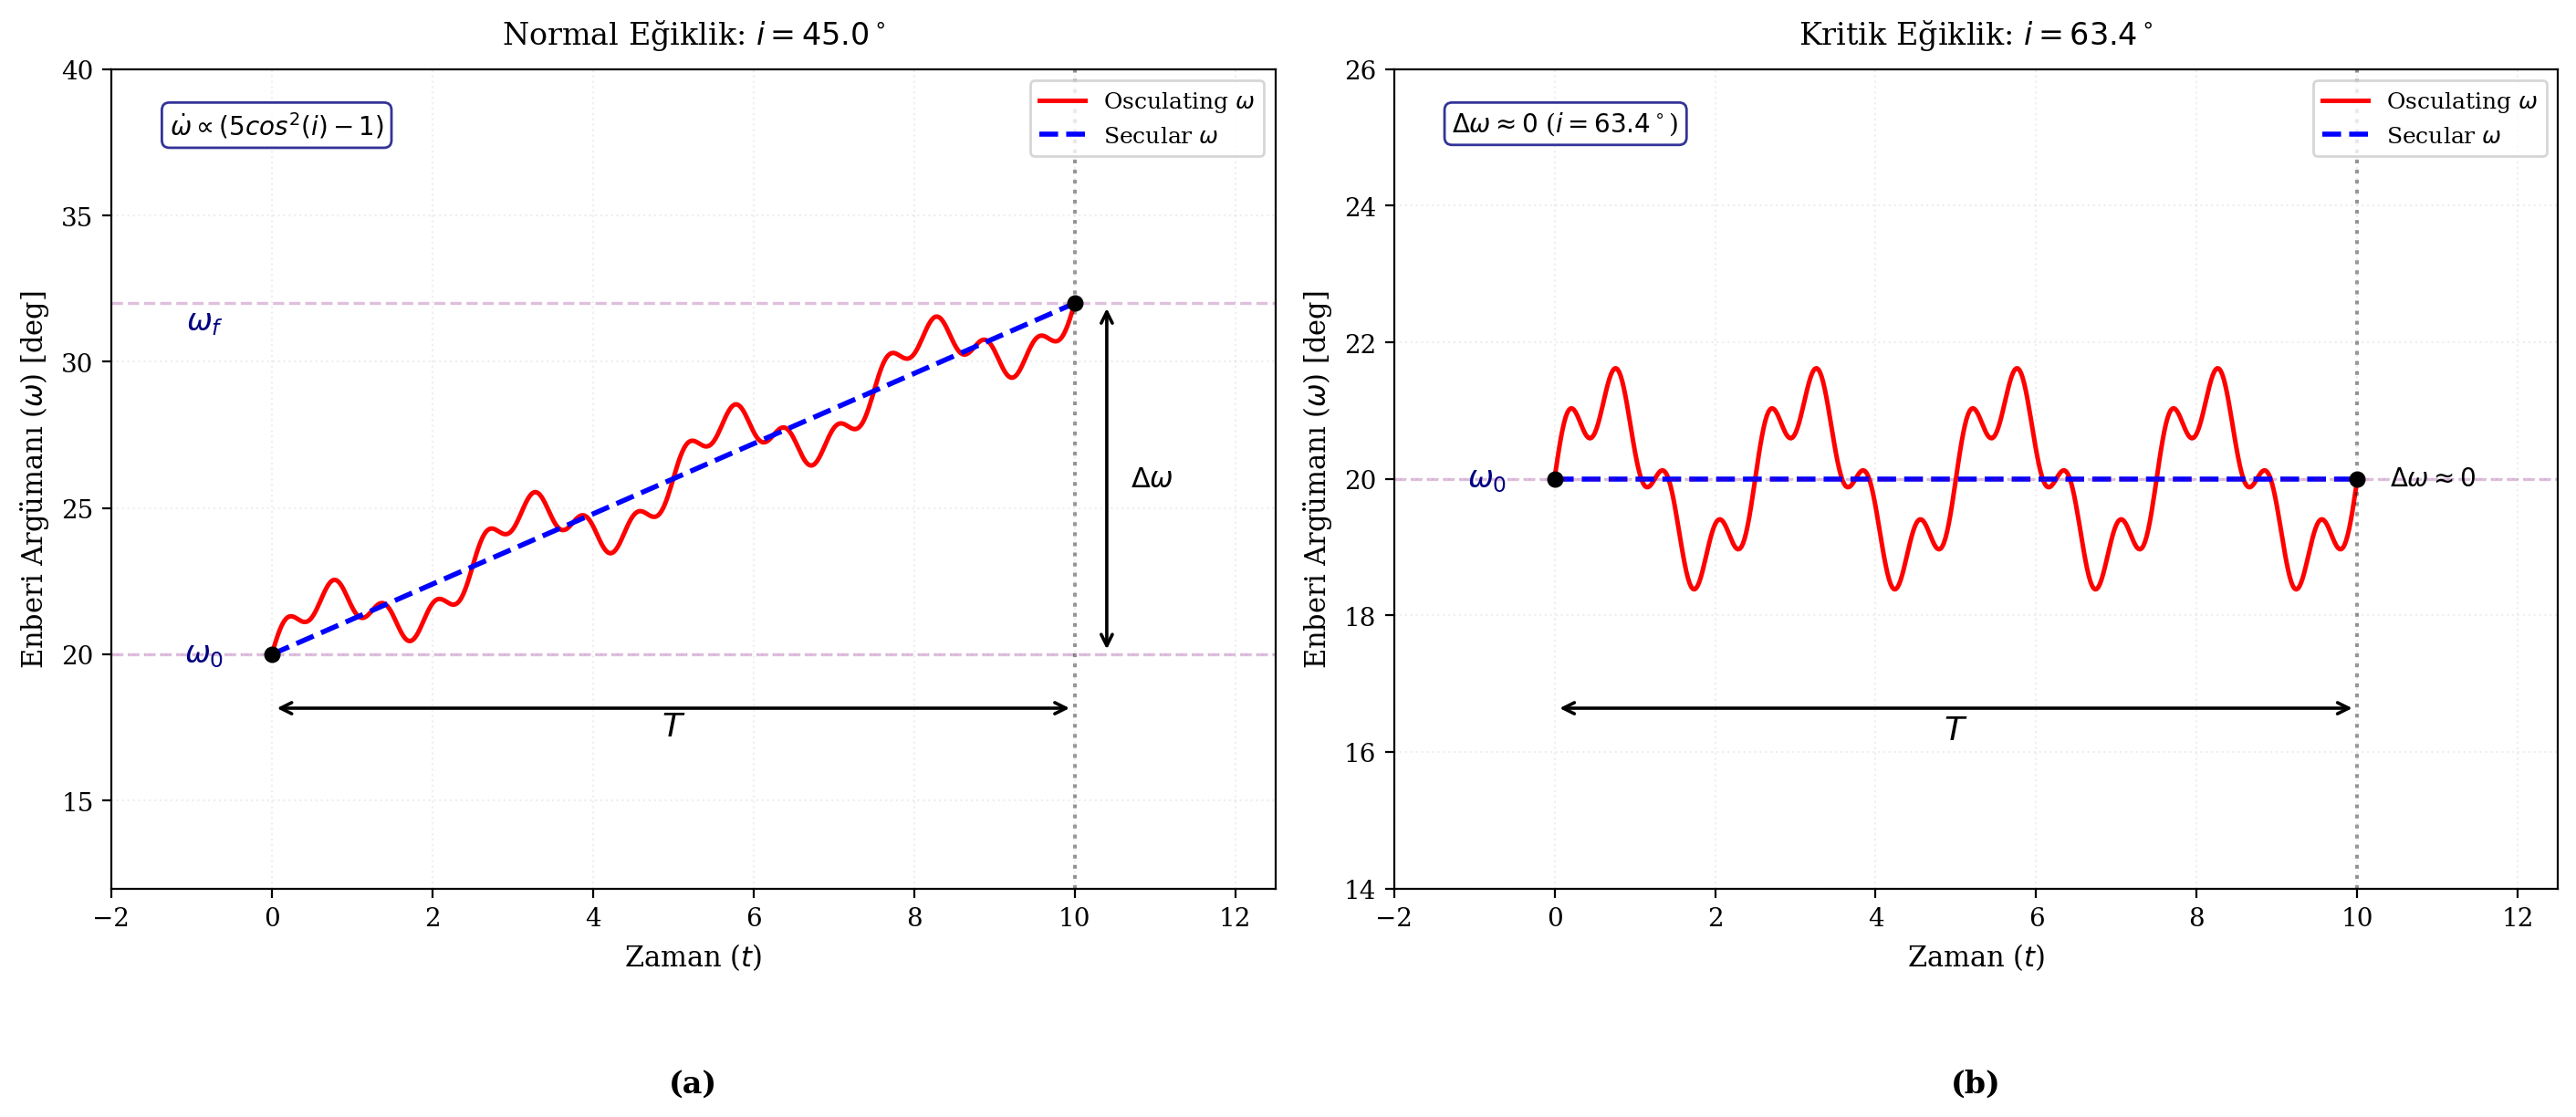
\includegraphics[width=0.95\linewidth]{Resimler/Dünya Modeli/Enberi Shift.png}
    \caption{J$_2$ etkisi altında enberi argümanı ($\omega$) değişimi: osculating (kırmızı) ve seküler/ortalama (mavi kesikli) bileşenlerin karşılaştırılması.
    (a) Genel bir eğiklikte $\Delta\omega \neq 0$ olup seküler drift lineerdir.
    (b) Kritik eğiklikte ($i\approx 63.4^\circ$) $5\cos^2 i - 1 \approx 0$ olduğundan seküler perigee drift yaklaşık sıfırdır; kısa-periyot salınımlar baskın kalır.}
    \label{fig:perigee_shift_j2}
\end{figure}

\noindent
\eqref{eq:omega_secular_J2}’nin en önemli sonucu, \textbf{kritik eğiklik} koşuludur:
\[
\big\langle \dot\omega \big\rangle \approx 0
\;\Rightarrow\;
5\cos^2 i -1 \approx 0
\;\Rightarrow\;
i \approx \arccos\sqrt{\frac{1}{5}} \approx 63.435^\circ.
\]
Bu durumda perigee argümanı uzun dönemde lineer drift göstermemeye yaklaşır; fakat osculating $\omega$
üzerindeki kısa-periyot salınımlar yine devam eder. Şekil \ref{fig:perigee_shift_j2}’de iki farklı eğiklik değeri için seküler ve gerçek bileşenlerin karşılaştırılması verilmiştir.




\medskip
Bu sonuçlar $J_2$ etkisinin tasarım açısından neden güçlü olduğunu açıkça gösterir:

\begin{itemize}
\item \textbf{İrtifa bağımlılığı:} Etki yaklaşık olarak $\left(R/p\right)^2$ ile ölçeklenir.
LEO’da ($p$ küçük) precesyonlar büyüktür; irtifa arttıkça hızla zayıflar.

\item \textbf{Eğim bağımlılığı:} $\dot{\Omega}$ doğrudan $\cos i$ ile, $\dot{\omega}$ ise $(5\cos^2 i-1)$ ile kontrol edilir. Dolayısıyla aynı irtifada dahi $ i $ seçimi ile istenen precesyon hızı ayarlanabilir.

\item \textbf{İşaret (yön) bilgisi:} $\dot{\Omega}$’nın negatif işareti, prograd yörüngelerde ($0^\circ<i<90^\circ$) düğüm gerilemesinin tipik olduğunu; retrograd yörüngelerde
($90^\circ<i<180^\circ$) ise işaretin tersine döndüğünü gösterir. Bu özellik, özellikle Güneş-eşzamanlı (SSO) yörünge tasarımında kritik rol oynar.

\end{itemize}

\begin{figure}[h]
    \centering
    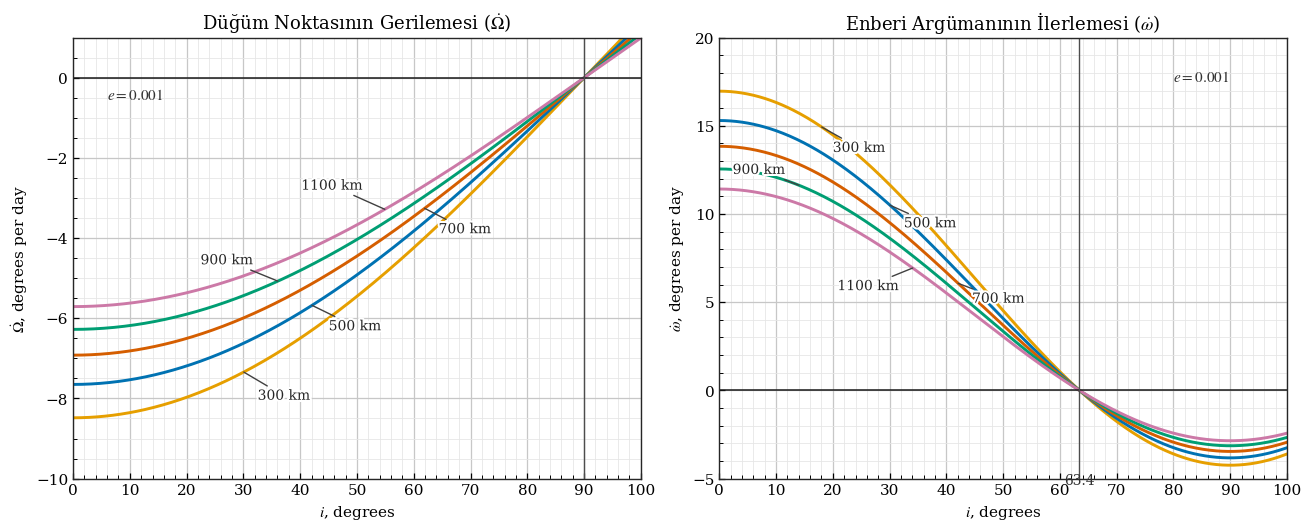
\includegraphics[width=1\linewidth]{Resimler/Dünya Modeli/RAAN ve Perigee V2.png}
    \caption{$J_2$ pertürbasyonuna bağlı olarak Düğüm Noktasının Gerilemesi ($\dot{\Omega}$) ve Enberi Argümanının İlerlemesi ($\dot{\omega}$) hızlarının yörünge eğikliği ve irtifaya göre değişimi ($e=0.001$).}
    \label{fig:j2_perturbations}
\end{figure}

Şekil~\ref{fig:j2_perturbations} incelendiğinde \cite{curtis2020orbital}, bu etkinin irtifa ve eğiklik ile olan hassas ilişkisi net bir biçimde görülmektedir. Soldaki grafikte, Düğüm Noktasının Gerilemesi ($\dot{\Omega}$) eğiklik ($i$) arttıkça azalmakta ve kutupsal yörüngelerde ($i=90^\circ$) sıfıra inmektedir. Düşük irtifalarda (örneğin 300 km) bu sürüklenme etkisi, yüksek irtifalara kıyasla çok daha belirgindir; bu durum $\dot{\Omega} \propto a^{-3.5}$ bağımlılığının doğrudan bir sonucudur. Sağdaki grafikte ise Enberi Argümanının İlerlemesi ($\dot{\omega}$), $i \approx 63.4^\circ$ değerinde işaret değiştirmektedir. Bu nokta \textbf{kritik eğim} olarak bilinir ve apsis hattının dönmesini durdurmak için Molniya gibi özel yörüngelerde stratejik olarak kullanılır. Grafikler, görev tasarımcısına istenen yörünge düzlemi presesyonunu elde etmek için hangi irtifa-eğiklik kombinasyonunun seçilmesi gerektiği konusunda doğrudan bir rehber sunar.



% -------------------- Lagrange Gezegen Denklemleri --------------
\subsection{Lagrange Gezegen Denklemleri (LPE)}\label{subsec:J2_LPE}

GVE yaklaşımı bozucu ivmeyi (RTN bileşenleri) doğrudan kullanırken, LPE yaklaşımı bozucu fonksiyon $\mathcal{R}$ üzerinden ilerler. $J_2$ etkisi \textbf{korunumlu} (\emph{konservatif}) bir potansiyelden türediği için, $\langle\dot{\Omega}\rangle$ ve $\langle\dot{\omega}\rangle$ gibi seküler oranlar LPE ile GVE’ye alternatif bir yoldan ve aynı sonuçlarla elde edilebilir. Kuvvet/ivme bileşenleri üzerinden çalıştığı için GVE, pertürbasyonun yönünü ve fiziksel etkisini yorumlama açısından çoğu zaman daha sezgiseldir; buna karşılık \textbf{konservatif alanlarda} LPE, potansiyelin ortalaması $\bar{\mathcal{R}}$ üzerinden ilerleyerek seküler dinamiği \textbf{daha sistematik} ve daha kompakt bir biçimde kurma avantajı sağlar. Bu nedenle, yöntembilimsel bütünlük sağlamak ve iki yaklaşımın eşdeğerliğini göstermek amacıyla, önce GVE ile elde edilen seküler sonuçlar bu kez LPE kullanılarak yeniden türetilecektir.


\subsubsection*{(i) Ortalama bozucu fonksiyon $\bar{\mathcal R}_{J_2}$}
$J_2$ bozucu fonksiyonu
\[
\mathcal R_{J_2} \;=\; -\frac{\mu R_E^2 J_2}{2r^3}\,(3\sin^2\phi-1),
\qquad \sin\phi=\sin i\sin u
\]
olduğundan, yörünge ortalaması alındığında (kısa-periyot terimler elenerek)
\begin{equation}
\boxed{
\bar{\mathcal R}_{J_2}
\;\triangleq\; \big\langle \mathcal R_{J_2}\big\rangle
\;=\; -\frac{\mu R_E^2 J_2}{4a^3(1-e^2)^{3/2}}\big(1-3\cos^2 i\big)
}
\label{eq:Rbar_J2}
\end{equation}
elde edilir. Bu ifade yalnızca $(a,e,i)$’ye bağlıdır ve açı değişkenlerine bağlı olmadığı için
seküler problemde $a,e,i$ sabit kalırken $\Omega$ ve $\omega$ sürüklenir.

\subsubsection*{(ii) Ortalama Lagrange denklemleri ile $\langle\dot\Omega\rangle$ ve $\langle\dot\omega\rangle$}
Ortalama bozucu fonksiyon kullanıldığında (yani $\bar{\mathcal R}$ ile),
klasik LPE’nin düğüm hattı ve perigee için pratik seküler formları:
\begin{subequations}\label{eq:LPE_secular_forms}
\begin{align}
\big\langle \dot\Omega \big\rangle \;&=\;
\frac{1}{n a^2\sqrt{1-e^2}\,\sin i}\,
\frac{\partial \bar{\mathcal R}}{\partial i},
\label{eq:LPE_Om}\\[4pt]
\big\langle \dot\omega \big\rangle \;&=\;
\frac{\sqrt{1-e^2}}{n a^2 e}\,
\frac{\partial \bar{\mathcal R}}{\partial e}
\;-\;
\frac{\cos i}{n a^2\sqrt{1-e^2}\,\sin i}\,
\frac{\partial \bar{\mathcal R}}{\partial i}.
\label{eq:LPE_om}
\end{align}
\end{subequations}
Şimdi \eqref{eq:Rbar_J2} ifadesinin türevlerini alalım. Önce $i$ türevi:
\[
\frac{\partial \bar{\mathcal R}_{J_2}}{\partial i}
=
-\frac{\mu R_E^2 J_2}{4a^3(1-e^2)^{3/2}}\,
\frac{\partial}{\partial i}\big(1-3\cos^2 i\big)
=
-\frac{\mu R_E^2 J_2}{4a^3(1-e^2)^{3/2}}\,(6\cos i\sin i).
\]
Bunu \eqref{eq:LPE_Om} içine koyarsak
\[
\big\langle \dot\Omega \big\rangle
=
\frac{1}{n a^2\sqrt{1-e^2}\sin i}
\Bigg(
-\frac{3\mu R_E^2 J_2}{2a^3(1-e^2)^{3/2}}\cos i\sin i
\Bigg)
=
-\frac{3}{2}J_2\,n\Big(\frac{R_E}{p}\Big)^2\cos i
\]
bulunur ve bu, GVE sonucu \eqref{eq:Omega_secular_J2} ile aynıdır.

Benzer şekilde $e$ türevi yalnızca $(1-e^2)^{-3/2}$ faktöründen gelir:
\[
\frac{\partial}{\partial e}\Big[(1-e^2)^{-3/2}\Big]
=
\frac{3e}{(1-e^2)^{5/2}}.
\]
Dolayısıyla
\[
\frac{\partial \bar{\mathcal R}_{J_2}}{\partial e}
=
-\frac{\mu R_E^2 J_2}{4a^3}\,
\frac{3e}{(1-e^2)^{5/2}}\,(1-3\cos^2 i).
\]
Bunu \eqref{eq:LPE_om} içine yerleştirip sadeleştirdiğimizde
\[
\big\langle \dot\omega \big\rangle
=
\frac{3}{4}J_2\,n\Big(\frac{R_E}{p}\Big)^2\big(5\cos^2 i - 1\big)
\]
elde edilir; bu da GVE sonucu \eqref{eq:omega_secular_J2} ile birebir aynıdır.

\subsubsection*{(iii) Sonuç: iki yol, aynı seküler fizik}
Özetle, $J_2$ gibi konservatif zonal pertürbasyonlarda:
\begin{itemize} \item GVE yaklaşımı $\mathbf a_{J_2}$’yi RTN bileşenlerine ayırarak doğrudan eleman driftlerini verir.
\item LPE yaklaşımı $\bar{\mathcal R}_{J_2}$ üzerinden kısmi türevlerle aynı seküler oranları üretir.
\end{itemize}
Bu noktadan sonra özel yörüngeler altbölümünde,
Sun-synchronous tasarımında \eqref{eq:Omega_secular_J2},
Molniya/kritik eğimde ise \eqref{eq:omega_secular_J2} temel denklemler olarak kullanılacaktır.


% ----------------- Daha Yüksek Zonal Terimler ----------------
\subsection{$J_3$, $J_4$ ve Daha Yüksek Zonal Terimler}
\label{subsec:J3_J4}

$J_2$'nin en baskın zonal bileşen olduğunu belirtmiştik. Örneğin
$J_3$ katsayısı, $J_2$'ye kıyasla yaklaşık $10^{-3}$ mertebesinde daha küçüktür; benzer biçimde $J_4$ da yaklaşık olarak $J_3$'e göre bir mertebe daha zayıf olup $10^{-6}$ mertebesine iner. Bu nedenle $J_3$, $J_4$ ve daha yüksek dereceli zonal terimler,
$J_2$'ye kıyasla oldukça küçük katkılar verir.

Yüksek hassasiyet gerektirmeyen tahmini analizlerde, bu küçük terimlerin büyüklüğü çoğu zaman \textbf{Kaula kuralı} ile mertebe düzeyinde tahmin edilir. Kaula kuralı, küresel harmonik katsayılarının genliğinin dereceyle yaklaşık olarak $\ell^{-2}$ ölçeğinde azaldığını öngören \textbf{ampirik} bir yaklaşımdır. Bu bağlamda, zonal terimler için tipik bir mertebe tahmini

\begin{equation}
|J_\ell| \;\sim\; \frac{|J_2|}{\ell^2}
\qquad (\ell\ge 3)
\label{eq:kaula_zonal}
\end{equation}
şeklinde verilebilir.

Buna karşın, yüksek hassasiyetli yörünge hesaplarında $J_3$, $J_4$ ve daha yüksek dereceli terimlerin tahmin edilmesi yeterli değildir; bu katsayıların güvenilir bir jeopotansiyel modelinden (örn.\ EGM/GRACE tabanlı modeller) alınarak nokta atışı şekilde
kullanılması gerekir. Çünkü Kaula kuralı yalnızca katsayıların \textbf{tipik büyüklük mertebesini} yakalar; yerel kütle anomalilerinin (dağlar, yoğunluk farkları vb.) uzaysal dağılımını ve bunların faz bilgisini temsil etmez. Dolayısıyla daha yüksek dereceli zonal terimler, Dünya'nın küresel şekline daha ince düzeltmeler ekleyerek özellikle uzun süreli propagasyonda
ve hassas görev analizlerinde uydunun izlediği yörüngeyi anlamlı ölçüde etkileyebilir. 

Genel olarak yüksek zonal terimlerin fiziksel anlamını ve yörünge elemanlarına yansımasını şöyle özetleyebiliriz:

\begin{itemize}
\item \textbf{$J_3$ (armut/pear-shape bileşeni):}
$J_3$ tek dereceli bir zonal terim olduğundan, kuzey--güney yönünde \textbf{asimetrik} bir katkı karakteri taşır. Bu yüzden etkileri çoğu zaman tamamen seküler bir sürüklenmeden ziyade
\textbf{uzun periyotlu} (long-period) salınımlar şeklinde görülür.
Özellikle eksantriklik $e$ ve perigee argümanı $\omega$ gibi elemanlarda, yörüngenin perigeesinin enleme göre konumlanmasına bağlı olarak yavaş değişimler/oscillasyonlar üretebilir.
(Çok küçük $e$’li neredeyse dairesel yörüngelerde bu etkinin gözlenmesi zorlaşır.)

\item \textbf{$J_4$ ve çift dereceli daha yüksek zonaller ($J_6,\dots$):}
Bu terimler, $J_2$’nin temsil ettiği ana basıklık üzerine
daha ince global şekil düzeltmeleri ekler. Etkileri genellikle $J_2$’ye göre daha küçük olsa da, \textbf{hassas yörünge propagasyonu} gerektiğinde (yüksek doğruluklu LEO görevleri,
uzun süreli yayılım, hassas yer izleme/ground-track gereksinimleri) ihmal edilemeyecek seviyeye çıkabilir.
Özellikle LEO’da, $J_2$ ile birlikte $J_4$ gibi terimler de $\Omega$ ve $\omega$ için ek precesyon bileşenleri ve elemanlarda daha karmaşık uzun periyot davranışları oluşturur.

\item \textbf{$J_5$ gibi tek dereceli daha yüksek zonaller ($J_5,J_7,\dots$):}
$J_3$’e benzer biçimde, kuzey--güney asimetri karakterli daha ince katkıları temsil ederler. Uygulamada çoğu zaman $J_2$ ve $J_4$ kadar ilk sırada yer almazlar; ancak uzun süreli propagasyon ve yüksek doğruluk hedeflerinde, özellikle belirli eğiklik/eksantriklik kombinasyonlarında uzun periyotlu etkiler biriktirebilirler.
\end{itemize}

\noindent
\textbf{Kısacası:}
Kaba görev analizlerinde çoğu zaman $J_2$ terimi baskındır ve yeterli bir ilk yaklaşım sunar; ancak hassasiyet gereksinimi arttıkça $J_3$, $J_4$ ve daha yüksek dereceli terimler
(başka bir deyişle model derecesi yükseldikçe) ihmal edilemeyecek düzeye gelir. Bu nedenle hangi zonal terimlerin modele dahil edileceği, \textbf{irtifa}, \textbf{zaman ufku} ve \textbf{istenen doğruluk} ile birlikte; gerekirse Kaula kuralı ile yalnızca mertebe düzeyinde bir ön değerlendirme yapılıp,
nihai analizde güvenilir jeopotansiyel katsayıları kullanılarak belirlenmelidir.




% =================== Özel Yörüngeler ====================
\newpage
\section{Özel Yörüngeler}
\label{sec:special_orbits}

Bu altbölümde, yerçekimi potansiyelinin düşük dereceli bileşenlerinin yörünge dinamiğinde neden bu kadar belirgin izler bıraktığına odaklanacağız. Bunun temel nedeni düşük dereceli terimler (özellikle zonaller), potansiyelin en büyük genlikli ve en geniş ölçekli sapmalarını taşır. Bu sapmalar her turda tekrar tekrar etki ettiği için, kısa zaman ölçeklerinde küçük görünen katkılar uzun vadede \textbf{birikimli} (\emph{seküler}) değişimlere dönüşebilir.

Bu çerçevede $J_2$ terimi, hem büyüklüğü hem de $\Omega$ (düğüm doğrusu) ve $\omega$ (apsis hattı / perigee argümanı) üzerinde ürettiği uzun dönemli, birikimli ortalama sürüklenmeler nedeniyle analizlerde birinci sıradadır. Özellikle $\Omega$ ve $\omega$’nun
ortalama precesyon hızları, görev tasarımında istenen yörünge geometrisini korumak veya istenen biçimde ayarlamak için birer kontrol parametresi gibi kullanılır. Aşağıda bu fikrin üç klasik yörünge ailesinde nasıl somutlaştığını görüyoruz.


% ---------------- Sun Synchronous -------------
\subsection*{2.4.1 \hspace{0.25em} Güneş-Eşzamanlı Yörüngeler (SSO)}
\label{subsec:sso}

Güneş-eşzamanlı yörüngelerde (Sun-Synchronous Orbit, SSO) amaç,
yörünge düzleminin uzaydaki yöneliminin (düğüm doğrusu, $\Omega$)
Güneş'in görünür yıllık hareketiyle \textbf{aynı ortalama açısal hızda}
dönmesini sağlamaktır.
Bu sayede uydu, aynı enlemden ardışık geçişlerinde yaklaşık aynı
\textbf{Yerel Güneş Zamanı} (Local Solar Time, LST) değerine sahip olur;
özellikle görüntüleme/uzaktan algılama görevlerinde aydınlatma koşulları
yıl boyunca daha \textbf{tutarlı} kalır.

Bu geometrik ilişki Şekil \ref{fig:sso_geometry}'de gösterilmiştir.
Düzlemin Güneş ile senkron kalması için düğüm presesyon hızı,
Dünya'nın Güneş etrafındaki ortalama açısal hızına eşitlenir:
\begin{equation}
\dot\Omega \;\approx\; \dot\Omega_{\odot}
\;\approx\; \frac{360^{\circ}}{365.25\ \text{gün}}
\;\approx\; 0.9856^{\circ}/\text{gün}.
\label{eq:sso_condition}
\end{equation}

\begin{figure}[h]
    \centering
    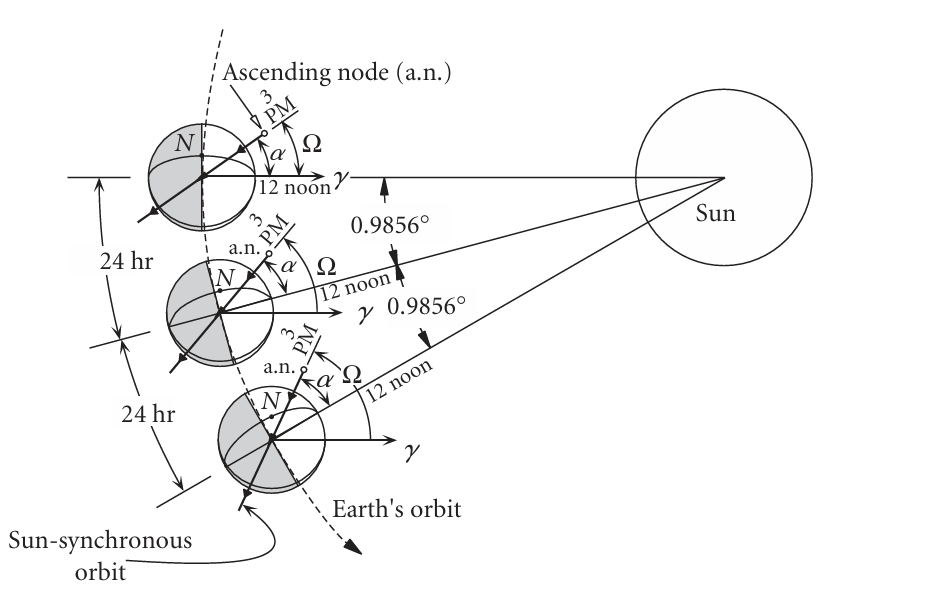
\includegraphics[width=0.85\linewidth]{Resimler/Dünya Modeli/SSO.png}
    \caption{Güneş-eşzamanlı yörüngenin geometrisi ve düğüm hattının Güneş ile senkron hareketi \cite{curtis2020orbital}.}
    \label{fig:sso_geometry}
\end{figure}

$J_2$ etkisi altında elde edilen seküler düğüm sürüklenmesi ifadesi \eqref{eq:Omega_secular_J2} dikkate alındığında,
\[
\big\langle \dot\Omega \big\rangle
\;=\; -\frac{3}{2}\,J_2\,n\Big(\frac{R_E}{p}\Big)^2\cos i,
\]

burada $n=\sqrt{\mu/a^3}$ ortalama hareketi, $p=a(1-e^2)$ ise yarı-parametreyi temsil eder.
Dolayısıyla $\langle \dot\Omega\rangle$ temel olarak $a$ (hem $n$ hem $p$ üzerinden), $e$ ( $p$ üzerinden)
ve $i$ ( $\cos i$ üzerinden) ile belirlenir.

SSO tasarımında hedef, düğüm hattının yıllık Güneş hareketine kilitlenmesidir; bu nedenle \eqref{eq:Omega_secular_J2} ile \eqref{eq:sso_condition} birlikte kullanılarak tasarım bağıntısı elde edilir:
\begin{equation}
\cos i
\;=\;
-\frac{2}{3}\;
\frac{\dot\Omega_{\odot}}{J_2\,n}\;
\Big(\frac{p}{R_E}\Big)^2.
\label{eq:SSO_design_relation}
\end{equation}

\begin{itemize}
    \item \textbf{İrtifa--eğim bağımlılığı:}
    $e\simeq 0$ için $p\simeq a$ ve $n\propto a^{-3/2}$ olduğundan,
    \eqref{eq:SSO_design_relation} yaklaşık olarak $\cos i \propto a^{7/2}$ ölçeğinde değişir.
    Bu yüzden pratikte bir \textbf{irtifa bandı} seçilir ve buna karşılık gelen $i$ belirlenir.

    \item \textbf{Retrograd gerekliliği:}
    \eqref{eq:Omega_secular_J2}'daki eksi işareti nedeniyle hedeflenen işaret için
    $\cos i<0$ olmalıdır; dolayısıyla SSO'lar tipik olarak
    $90^{\circ}<i<180^{\circ}$ aralığında \textbf{retrograd} seçilir.
\end{itemize}

Pratikte SSO'lar çoğunlukla düşük eksantriklikli LEO yörüngeleridir ($e\approx 0$).
Ayrıca atmosferik sürükleme zamanla $a$'yı azalttığından,
$\langle \dot\Omega\rangle$ da yavaşça değişebilir; hassas LST korunumu için
operasyonel düzeltmeler gerekebilir.

Sonuç olarak SSO, $J_2$ kaynaklı düğüm presesyonunun bir ``hata'' değil,
doğru seçilmiş $(a,i,e)$ ile görev gereksinimini sağlayan
\textbf{bilinçli bir tasarım aracı} olarak kullanıldığı klasik bir örnektir.




% --------------- Molniya Yörüngeleri -----------------
\subsection*{2.4.2 \hspace{0.25em} Molniya Yörüngeleri}
\label{subsec:molniya}

Molniya tipi yörüngeler, yüksek dışmerkezlikli ve yüksek eğimli (eliptik) yörüngelerdir.
Bu sınıfta temel amaç, enöte civarındaki uzun kalış bölgesinin (dolayısıyla kapsama geometrisinin)
zamanla yer değiştirmemesidir. Bu nedenle tasarımda özellikle apsis hattının yönelimi ve
\textbf{enberi argümanının} $\omega$ seküler sürüklenmesi kritik hale gelir.

\begin{tcolorbox}[
    colback=blue!8!white,
    colframe=blue!35!black,
    boxrule=0.6pt,
    arc=2mm,
    left=4pt,
    right=4pt,
    top=4pt,
    bottom=4pt,
    title=\small\textbf{Tarihsel ve Operasyonel Motivasyon}
]
Rus fırlatma sahalarının büyük bölümü $45^\circ$ enleminin üzerindedir
(kuzeydeki Plesetsk $\sim62.8^\circ$N).
Bu enlemlerden jeostasyoner yörüngeye (GEO) doğrudan erişim,
Ekvator düzlemiyle olan eğim farkı nedeniyle genellikle \textbf{pahalı bir düzlem değiştirme} (\emph{plane change}) manevrası gerektirir. Bu tür bir düzlem değiştirme manevrasının yaklaşık hız gereksinimi
\[
\Delta V_{\text{pc}} \;\approx\; 2\,V\,\sin\!\Big(\frac{\Delta i}{2}\Big),
\]
şeklinde ifade edilebilir; burada $V$ yörünge hızı, $\Delta i$ ise gerekli eğim değişimini temsil eder.
Yüksek irtifa ve hızlarda bu maliyet hızla büyür. Öte yandan GEO uyduları yüksek kuzey enlemlerini düşük yükselim açısıyla gözlediği için, kapsama geometrisi ve link bütçesi dezavantajlı hale gelir. Bu nedenle Sovyet/Rus haberleşme mimarisinde, 12 saat periyotlu ve yüksek eliptik (HEO) yörüngeler, yüksek enlemler üzerinde uzun süreli görünürlük sağlamak için etkili bir çözüm olarak öne çıkmıştır \cite{curtis2020orbital}.
\end{tcolorbox}


\eqref{eq:omega_secular_J2} ifadesi hatırlanırsa, $J_2$ kaynaklı ortalama enberi precesyonu
\begin{align*}
\big\langle \dot\omega \big\rangle
\;=\; \frac{3}{4}\,J_2\,n\Big(\frac{R_E}{p}\Big)^2\big(5\cos^2 i - 1\big)
\end{align*}
şeklindedir. Molniya tasarımında hedef, enöte bölgesinin seçilen yarımkürede kararlı kalması için
$\langle\dot\omega\rangle$ değerini sıfıra (veya sıfıra yakın) indirmektir. Bu da
\begin{equation}
5\cos^2 i-1=0
\quad\Longrightarrow\quad
i \approx 63.435^\circ \ \ (\text{veya }116.565^\circ)
\label{eq:critical_inclination}
\end{equation}
koşulunu verir. Bu değer \textbf{kritik eğim} olarak bilinir; kritik eğimde $J_2$ etkisinin $\omega$ üzerindeki seküler (ortalama) bileşeni bastırılır ve apsis hattının yönelimi uzun vadede daha kararlı hale gelir. Bu nedenle Molniya tasarımlarında eğim çoğunlukla kritik eğim civarında seçilir ($i \approx 63.435^\circ$); böylece apsis hattının uzun vadeli yönelimi korunarak enöte bölgesindeki kapsama geometrisi kararlı tutulur.


\begin{figure}[h]
    \centering
    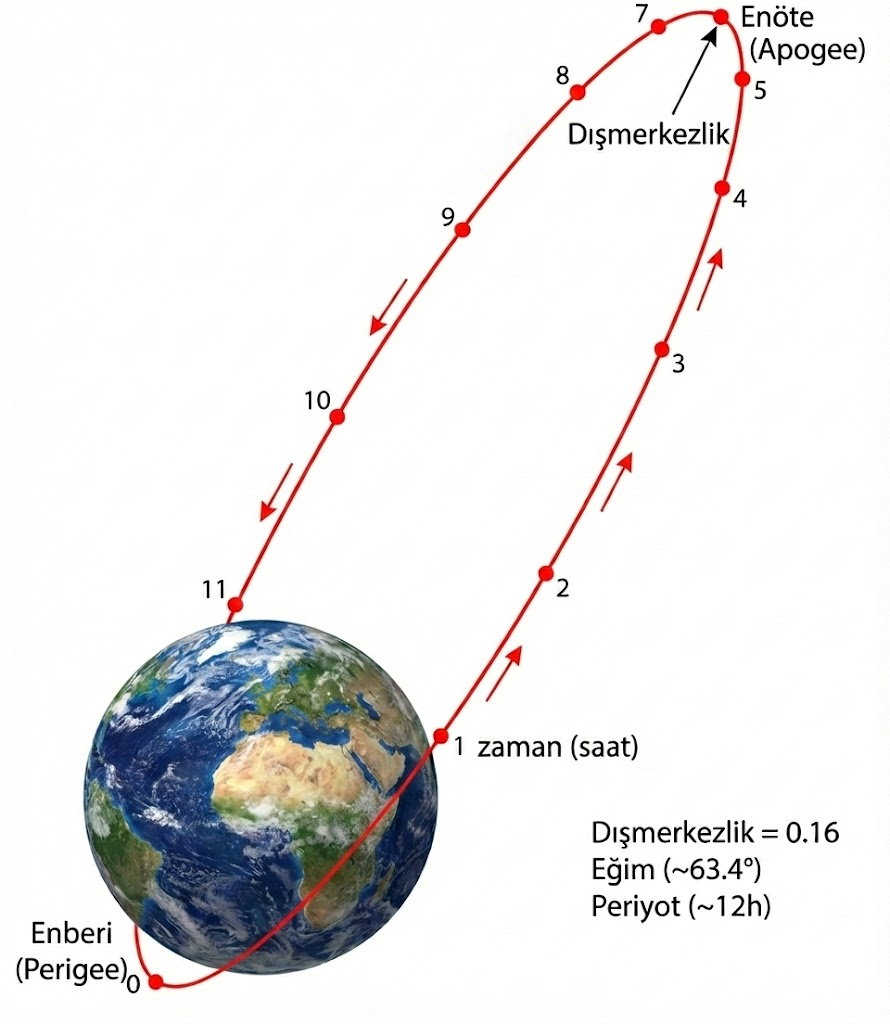
\includegraphics[width=0.5\linewidth]{Resimler/Dünya Modeli/Molniya Yörüngesi.png}
    \caption{Molniya tipi 12 saatlik eliptik yörüngede uydunun yörünge boyunca konumu. Enöte civarında hızın azalması nedeniyle zaman işaretleri sıklaşır; bu, uydunun periyodun büyük kısmını enöte yakınında geçirerek yüksek enlemlere uzun süreli kapsama sağlamasının görsel bir göstergesidir.}
    \label{fig:molniya_orbit}
\end{figure}

Şekil~\ref{fig:molniya_orbit}, kapsama avantajının dinamik nedenini görselleştirir:
uydu enöte civarında daha yavaş ilerlediği için eşit zaman aralıklarıyla işaretlenen konum noktaları
enöte yakınında daha sık, enberi yakınında ise daha seyrek görünür.
Bu dağılım Kepler’in ikinci yasasının doğrudan sonucudur ve uydunun periyodun önemli bir kısmını
enöte çevresinde geçirdiğini gösterir. Ayrıca $T\simeq 12$ saat seçimi,
yer izi ve yer istasyonu geometrisi açısından günlük tekrar eden bir örüntü sağlayarak operasyonel planlamayı kolaylaştırır.


% ---------------- Tundra Yörüngeleri-------------
\newpage
\subsection*{2.4.3 \hspace{0.25em} Tundra Yörüngeleri}
\label{subsec:tundra}

Tundra yörüngeleri, Molniya’daki temel prensibi (apsis hattını kararlı tutma ve enöteyi
istenen yarımküreye ``kilitleme'') \textbf{yaklaşık 1 yıldız günü (sidereal day) periyot}
çevresinde uygular. Bu sınıf, özellikle \textbf{yüksek enlemlere hizmet veren haberleşme}
görevlerinde, jeostasyoner yörüngelerin yüksek enlemlerdeki düşük yükselim açısı
dezavantajını azaltmak amacıyla geliştirilmiş yüksek eliptik
\emph{jeosenkron} (HEO--GSO) yörüngelerdir.

Tundra tasarımının merkezinde \textbf{apogee dwell} olgusu yer alır:
uydu enöte civarında belirgin biçimde yavaşladığı için yörünge periyodunun büyük bir
kısmını seçilen coğrafi bölge üzerinde geçirir.
Periyot bir güne yaklaştığında bu uzun kalış her gün yaklaşık aynı yerel zamanlarda
tekrar eder; bu durum yer istasyonu planlamasını ve görünürlük sürekliliğini
operasyonel açıdan avantajlı hâle getirir.

Dinamik açıdan Tundra yörüngeleri iki temel koşula dayanır:
\begin{itemize}
    \item \textbf{Periyot (jeosenkronluk):}
    Periyot $T \approx 1$ yıldız günü olacak şekilde yarı-büyük eksen $a$ seçilir.
    Bu seçim, yörüngenin Dünya’ya göre günlük tekrar eden bir yer izi üretmesini sağlar.

    \item \textbf{Eğim (J$_2$ ile apsis kararlılığı):}
    $J_2$ kaynaklı seküler apsis sürüklenmesini azaltmak için eğim çoğunluklakla
    \textbf{kritik eğime} yakın seçilir ($i \approx 63.4^\circ$ veya tamamlayanı).
    Böylece $\dot{\omega}$’nun seküler bileşeni bastırılarak apsis hattının
    uzaydaki yönelimi uzun vadede korunur.
\end{itemize}

Pratik uygulamalarda Tundra yörüngeleri \textbf{orta--yüksek dışmerkezlik} ile tasarlanır;
tipik olarak $e \sim 0.2{-}0.3$ aralığı, enöte civarında yeterli ``loiter'' süresi
sağlarken kapsama geometrisini de operasyonel olarak elverişli kılar.
Bu sayede uydu, seçilen boylam/enlem bandı üzerinde
\textbf{yüksek yükselim açısıyla} uzun süre görünür kalabilir.

\begin{figure}[h]
    \centering
    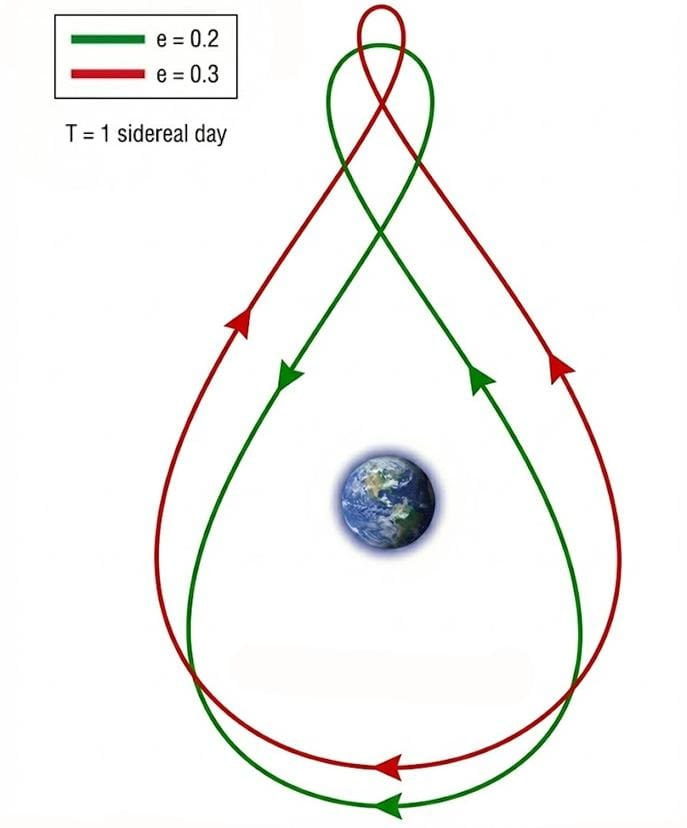
\includegraphics[width=0.5\linewidth]{Resimler/Dünya Modeli/Tundra.jpeg}
    \caption{Dünya ile dönen (Earth-fixed) referans çerçevesinde,
    farklı dışmerkezliklere ($e=0.2$ ve $e=0.3$) sahip Tundra yörüngelerinin
    yer izi (analemma) görünümü.}
    \label{fig:tundra_analemma}
\end{figure}

Şekil~\ref{fig:tundra_analemma}, iki farklı dışmerkezlik değerine sahip Tundra
yörüngesinin Dünya’ya göre algılanan yer izini göstermektedir.
Dünya ile dönen (\emph{Earth-fixed}) bir referans çerçevesinde,
yörünge kapalı bir ``8'' (analemma) biçimi oluşturur.
Bu şekil, Dünya’nın günlük dönüşü ile yörüngenin jeosenkron periyodunun
birlikte etkisinin doğrudan sonucudur.
Buna karşılık, eylemsiz (\emph{Earth-centered inertial}) referans çerçevesinde
Tundra yörüngesi basit bir elips olarak tanımlanır.

Şekilden de görüldüğü üzere, dışmerkezlik arttıkça enöte civarındaki
\textbf{apogee dwell} süresi artmakta ve analemmanın ilgili yarımküredeki
halkası daha baskın hâle gelmektedir.
Bu durum, Tundra yörüngelerinin belirli bir coğrafi bölge üzerinde
uzun süreli ve yüksek yükselimli görünürlük sağlamasının
geometrik ve dinamik temelini açıkça ortaya koyar.

Sonuç olarak Tundra yörüngeleri, $J_2$ kaynaklı apsis sürüklenmesini
\emph{tasarım lehine} kullanarak,
jeosenkron periyot ile enöte kalışını birleştiren ve
belirli bir bölge üzerinde sürekliliğe yakın kapsama sağlamaya odaklanan
özel bir yüksek eliptik yörünge ailesidir.


% ------------------ Özet -------------------
\subsection*{2.4.4 \hspace{0.25em} Özet}
Güneş-eşzamanlı, Molniya ve Tundra örnekleri, $J_2$ kaynaklı seküler sürüklenmelerin yalnızca
``istenmeyen pertürbasyonlar'' olmadığını gösterir. Uygun $(a,e,i)$ seçimiyle
$\Omega$ ve $\omega$ üzerindeki ortalama precesyonlar \textbf{hedeflenebilir} veya
\textbf{bastırılabilir}; böylece görev gereksinimlerine uyumlu \textbf{özel yörünge} aileleri
tasarlanır. Bu bakımdan $J_2$, pertürbasyon modellemesinin ötesinde,
yörünge geometrisini uzun vadede yönlendiren bir \textbf{tasarım parametresi} gibi davranır.
Aşağıdaki tabloda bu üç yörünge ailesinin temel özellikleri karşılaştırılmıştır.

\medskip
\begin{table}[h]
\centering
\captionsetup{skip=6pt}
\renewcommand{\arraystretch}{1.25}
\setlength{\tabcolsep}{6pt}
\begin{tabular}{p{2.6cm} p{3.4cm} p{3.6cm} p{5.2cm}}
\hline
\textbf{Yörünge} &
\textbf{Ana hedef} &
\textbf{$J_2$ ile kurulan şart} &
\textbf{Tipik seçimler ve sonuç} \\
\hline
Güneş-Eşzamanlı (SSO) &
Yerel Güneş Zamanını (LST) yaklaşık sabit tutmak &
Düğüm precesyonu hedeflenir:
$\langle\dot\Omega\rangle \approx \dot\Omega_{\odot}$ &
LEO, düşük $e$; retrograd eğim ($i>90^\circ$).
Yıl boyunca benzer aydınlatma koşulları. \\
\hline
Molniya (HEO) &
Yüksek enlemlerde uzun süreli kapsama (enöte loiter) &
Apsis sürüklenmesi bastırılır:
kritik eğimde $\langle\dot\omega\rangle \approx 0$ &
$T\approx 12$ saat; yüksek $e$;
$i\approx 63.4^\circ$ (veya $116.6^\circ$).
Enöte civarında belirgin ``dwell'' süresi. \\
\hline
Tundra (HEO--GSO) &
Belirli bir boylam bölgesi üzerinde günlük tekrar eden uzun görünürlük &
$\langle\dot\omega\rangle$ azaltılır (kritik eğim civarı) ve enöte yönelimi korunur &
$T\approx 1$ yıldız günü; $e\sim 0.2{-}0.3$;
$i$ kritik eğime yakın.
Earth-fixed çerçevede analemma (``8'') yer izi. \\
\hline
\end{tabular}
\caption{SSO, Molniya ve Tundra yörüngelerinin $J_2$ ile ilişkili tasarım hedefleri ve tipik özellikleri.}
\label{tab:special_orbits_summary}
\end{table}




% ============== Potansiyel Ölçümleri ve Tarihçesi ===============
\newpage
\section{Potansiyel Ölçümleri ve Tarihçesi}
\label{sec:measurements_history_estimation}

Şimdiye kadar, yerçekimi potansiyelinin küresel harmonikler cinsinden nasıl temsil edildiğini gördük. Ancak Dünya özelinde bu katsayılara duyulan gereksinimin hangi fiziksel ve tarihsel nedenlerle ortaya çıktığı açıklığa kavuşturulmalıdır.
Bu bağlamda, \eqref{eq:earth_potential} denkleminde yer alan
$\bar C_{\ell,m}$ ve $\bar S_{\ell,m}$ katsayılarının nasıl bulunduğu incelenecektir.


% --------------- Modellerin Tarihçesi ------------
\subsection{Dünya Yerçekimi Modellerinin Tarihçesi}
\label{subsec:history_short}

Küresel yerçekimi modellerinin gelişimi, insanlığın yapay uyduları yörüngeye yerleştirmesiyle
doğrudan ivme kazanmıştır. Erken dönem uyduların yörüngelerinde gözlenen beklenmedik
sapmalar, Dünya’nın kütle dağılımının basit bir küresel modelle açıklanamayacağını ortaya koymuştur.
Ölçüm teknikleri ve izleme hassasiyeti geliştikçe, yalnızca düşük dereceli bileşenler değil,
daha ince uzaysal ayrıntılar ve hatta zamanla değişen kütle etkileri de görünür hale gelmiştir.

\begin{itemize}
\item \textbf{1957--1960’lar (ilk yapay uydular):}
Sputnik ve onu izleyen erken dönem uyduların yörüngelerinde gözlenen düğüm ve apsis sürüklenmeleri, yerçekimi alanındaki düşük dereceli zonal terimlerin (özellikle $J_2$) baskın rolünü açıkça ortaya koydu. Bu dönemde Dünya’nın basıklığı, ilk kez yalnızca jeodezik ölçümlerle değil, doğrudan yörünge dinamiği üzerinden nicel olarak doğrulanmış oldu.

\item \textbf{1970’ler ve LAGEOS (1976):}
LAGEOS uydularının lazerle menzillenmesi (SLR), yörünge konumunun milimetre mertebesinde izlenmesini mümkün kıldı. Atmosferik sürüklemenin ihmal edilebilir olduğu bu yüksek irtifa
uyduları, düşük dereceli ve uzun dalga boylu yerçekimi bileşenleri için son derece güvenilir referanslar sundu ve küresel modellerin temelini sağlamlaştırdı.

\item \textbf{2000 ve CHAMP:}
CHAMP göreviyle birlikte GNSS/GPS tabanlı hassas yörünge belirleme teknikleri olgunlaştı. Bu sayede yalnızca düşük dereceler değil, orta dereceli harmonik bileşenler de daha güvenilir biçimde çözümlenebildi. CHAMP, dinamik uydu izleme ile gravite modellemenin modern çağına geçişte kritik bir ara basamak olarak kabul edilir.

\item \textbf{2002 ve GRACE:}
GRACE görevi, iki uydu arasındaki bağıl mesafedeki mikrometre düzeyindeki değişimleri ölçerek yerçekimi alanını benzeri görülmemiş bir hassasiyetle haritaladı. Bu yaklaşım, yerçekimi alanının yalnızca statik bir nicelik olmadığını; buz tabakaları, yeraltı suyu, okyanus ve kara kütle değişimleri nedeniyle
\textbf{zamansal olarak değiştiğini} doğrudan gözler önüne serdi.

\item \textbf{2009 ve GOCE:}
GOCE uydusu üzerindeki gradiyometre, yerçekimi ivmesinin uzaysal türevlerini doğrudan ölçerek statik alanın kısa dalga boylu (yüksek dereceli) ayrıntılarını büyük ölçüde iyileştirdi.
Bunun sonucunda jeoit modelleri daha keskin, daha düzgün ve daha yüksek çözünürlüklü hale geldi; özellikle bölgesel jeodezi ve okyanus dinamiği uygulamaları önemli kazanımlar elde etti.

\item \textbf{2018 ve GRACE-FO:}
GRACE-FO görevi, GRACE ile başlatılan zamansal yerçekimi gözlemlerini sürdürerek uzun dönemli eğilimlerin (buz erimesi, su bütçesi değişimleri gibi) daha güvenilir biçimde izlenmesini sağladı. Lazer interferometre gibi yeni teknolojilerle ölçüm hassasiyeti daha da artırıldı ve zamansal gravite gözlemlerinin sürekliliği garanti altına alındı.
\end{itemize}

\medskip
\noindent
\textbf{Bugün gelinen nokta:}
Günümüzde Dünya yerçekimi alanı, düşük dereceli zonal terimlerden
yüksek dereceli ve zamana bağlı bileşenlere kadar geniş bir yelpazede yüksek doğrulukla modellenebilmektedir. EGM2008, EIGEN, ITSG ve benzeri modern jeopotansiyel modelleri, SLR, GNSS, GRACE/GRACE-FO, GOCE ve altimetri verilerinin çoklu veri birleşimiyle üretilmekte; böylece hem statik alanın ince
uzaysal ayrıntıları hem de zamansal kütle değişimleri güvenilir biçimde temsil edilebilmektedir. Bu gelişmeler, yalnızca yörünge mekaniği ve görev tasarımı açısından değil, iklim değişikliği, su kaynakları, buz tabakalarının evrimi ve jeodinamik süreçlerin izlenmesi açısından da yerçekimi modellerini vazgeçilmez
bir bilimsel araç haline getirmiştir.

% ------------------- EGM Ailesi -----------------
\subsection*{EGM ailesi ve çözünürlük seviyeleri}
\label{subsec:EGM_family}

EGM (Earth Gravitational Model) ailesi gibi küresel yerçekimi modelleri,
$\bar C_{\ell, m}, \bar S_{\ell, m}$ küresel harmonik katsayılarının standartlaştırılmış bir ``kataloğu'' olarak yayımlanır. Bir modelin uzaysal ayrıntı kapasitesi çoğu zaman
\textbf{maksimum derece ve mertebe} ile özetlenir:
\[
\ell_{\max} = m_{\max},
\]
yani potansiyel açılımının hangi dereceye kadar genişletildiği.
Genel olarak $\ell_{\max}$ büyüdükçe model,
Dünya üzerindeki daha kısa dalga boylu (daha küçük ölçekli)
kütle ve jeoit yapılarının temsilini mümkün kılar.

EGM ailesindeki başlıca modeller ve derece seviyeleri şu şekildedir:
\begin{itemize}
\item \textbf{EGM84:} $\ell_{\max}=180$,
\item \textbf{EGM96:} $\ell_{\max}=360$,
\item \textbf{EGM2008:} $\ell_{\max}=2160$
(Bölgesel uzatmalarla daha yüksek dereceler).
\end{itemize}

Pratik açıdan model derecesinin anlamı iki temel noktada ortaya çıkar:

\begin{itemize}
\item \textbf{Derece--uzaysal ölçek ilişkisi:}
Küresel harmoniklerin temsil ettiği karakteristik yatay dalga boyu,
yaklaşık olarak
\[
\lambda \sim \frac{2\pi R_E}{\ell}
\]
ile ölçeklenir.
Dolayısıyla $\ell_{\max}$ arttıkça modelin yatay çözünürlüğü artar.
Ancak bu artış, her coğrafi bölgede eşit veri kalitesi olduğu anlamına gelmez;
veri yoğunluğu zayıf alanlarda yüksek dereceli terimler
daha belirsiz olabilir.

\item \textbf{İrtifa ve sönüm etkisi:}
Yüksek dereceli terimlerin katkısı,
uydu irtifası arttıkça $(R_E/r)^{\ell}$ faktörü nedeniyle hızla zayıflar.
Bu nedenle alçak yörüngelerde (özellikle LEO)
yüksek dereceli terimler anlamlı hale gelirken,
yüksek irtifalarda düşük dereceli bileşenler baskın kalır.
\end{itemize}

Buna ek olarak, derece yükseldikçe tahmin edilmesi gereken katsayı sayısı
yaklaşık olarak $(\ell_{\max}+1)^2$ ile artar.
Bu durum daha fazla ve daha çeşitli gözlem verisi gerektirir;
ayrıca ölçüm gürültüsünün yüksek derecelerde baskın hale gelmemesi için
kestirim sürecinde düzenlileştirme (regularizasyon),
a priori bilgi ve kalite kontrol adımları kritik rol oynar.

Sonuç olarak uygulamada model seçimi,
yalnızca ``en büyük $\ell_{\max}$ en iyidir'' anlayışıyla yapılmaz.
Hedeflenen irtifa, görev süresi ve istenen doğruluk düzeyine bağlı olarak,
tam model yerine uygun bir dereceye kadar
\emph{kesilmiş} (truncated) bir jeopotansiyel model kullanmak
çoğu zaman daha dengeli ve güvenilir bir yaklaşımdır.



% ----------------- C ve S hesaplama -------------
\section{$\bar C_{\ell,m},\bar S_{\ell,m}$ katsayıları nasıl kestirilir?}
\label{sec:how_CS_estimated}

Tarihsel gelişim incelendikten sonra, bu bölümde
$\bar C_{\ell,m}$ ve $\bar S_{\ell,m}$ küresel harmonik katsayılarının günümüzde hangi ölçüm türlerine dayalı olarak ve hangi sayısal yöntemlerle kestirildiği ele alınmaktadır.
Önce yerçekimi alanına duyarlı başlıca gözlem kaynakları özetlenecek, ardından bu gözlemlerin dinamik yörünge modelleriyle birleştirilerek katsayıların ters problem çerçevesinde nasıl hesaplandığı açıklanacaktır.


\subsection{Ölçüm Yöntemleri}
Başlıca veri kaynakları şunlardır:

\begin{itemize}
\item \textbf{Yer temelli gravite ölçümleri:}
Gravimetre ölçümlerinden elde edilen $g$ anomalileri ve bunlardan türetilen jeoit/gravite alan ürünleri, özellikle karasal bölgelerde bölgesel ayrıntılara güçlü katkı sağlar. Yer istasyonlarının iyi tanımlı geometrisi önemli bir avantajdır; ancak okyanuslar, erişimi zor alanlar ve düzensiz istasyon dağılımı nedeniyle küresel kapsam sınırlı kalabilir.

\item \textbf{SLR (Satellite Laser Ranging):}
Uyduya lazer menzili ölçülerek yörünge çok yüksek doğrulukla bağlanır. LAGEOS benzeri uydular sayesinde düşük dereceli bileşenler (uzun dalga boyu; özellikle $J_2$ ve yakın terimler) üzerinde son derece güçlü bir kısıt sağlanır. Atmosferik sürüklemenin ihmal edilebilir olduğu yüksek irtifa SLR uyduları,
``temiz dinamik'' yörünge verisi sunmaları nedeniyle temel referans veri kaynağıdır.

\item \textbf{GNSS/Doppler izleme:}
GNSS (GPS, Galileo vb.) alıcıları ile Doppler ve menzil türü izleme verileri, uydunun konum ve hızının hassas belirlenmesini sağlar. Bu sayede yörünge üzerindeki küçük ivme farkları daha net ortaya çıkar ve küresel harmonik katsayılarının kestirimi güçlenir. Uygulamada bu veri türü çoğu zaman hassas yörünge belirleme (POD) sürecinin ana girdisidir.

\item \textbf{Uydu--uydu izleme (GRACE/GRACE-FO):}
İki uydu arasındaki menzil değişimi ve menzil hızı (K/Ka-band ya da lazer interferometresi) ölçülür. Bu ölçümler yerçekimi alanının orta dalga boylu yapıları için son derece hassastır.
En önemli avantajı, yalnızca statik alanı değil; su döngüsü, buz kütlesi ve yeraltı suyu gibi \textbf{zamansal kütle değişimlerini} aylık hatta haftalık ölçeklerde izleyebilmesidir.

\item \textbf{Gradiyometri (GOCE):}
Yerçekimi ivmesinin uzaysal türevleri (gradyanları) doğrudan ölçülür. Bu veri türü kısa dalga boylu (yüksek derece) statik alan ayrıntılarının belirlenmesinde son derece etkilidir ve yüksek çözünürlüklü jeoit modellerinin temel bileşenlerinden biridir. Bununla birlikte, düşük dereceler için tek başına yeterli olmadığından genellikle SLR ve GRACE verileriyle birlikte kullanılır.

\item \textbf{Altimetri:}
Radar altimetreleri ile deniz yüzeyi yüksekliği ölçülür.
Uzun dönemli ortalama deniz yüzeyi, dinamik okyanus etkileri ayrıştırıldıktan sonra
jeoitin dolaylı bir gözlemi olarak kullanılır.
Bu veri, özellikle okyanuslar üzerindeki orta ve kısa dalga boylu gravite bileşenlerine
katkı sağlar; ancak akıntılar, rüzgâr ve dalga etkilerinin modellenmesi kritik önemdedir.
\end{itemize}

Bu veri türlerinin her biri farklı uzaysal ve zamansal ölçeklere duyarlıdır: bazıları uzun dalga boyunu (düşük $\ell$), bazıları kısa dalga boyunu (yüksek $\ell$), bazıları ise zamanla değişen bileşenleri daha iyi temsil eder. Bu nedenle modern jeopotansiyel modelleri, farklı veri setlerini \textbf{çoklu veri birleşimi} (\emph{data fusion}) yaklaşımıyla bir araya getirir. Veri ağırlıkları, ölçüm gürültüsü ve model belirsizlikleri EKK çerçevesinde birlikte değerlendirilerek tutarlı ve yüksek doğruluklu bir katsayı kümesi elde edilir.


% ------------- Sayısal Hesaplama Yöntemi ---------------
\subsection{Sayısal Hesaplama Yöntemi}

$\bar C_{\ell,m}$ ve $\bar S_{\ell,m}$ katsayıları doğrudan ölçülebilen nicelikler değildir.
Bu katsayılar, yerçekimi alanının uydu yörüngeleri üzerindeki etkisini açıklayan
dinamik modeller ile çeşitli jeodezik gözlemleri ilişkilendiren bir
\textbf{ters problem} çözümü yoluyla kestirilir.
Uygulamada en yaygın yaklaşım, \textbf{En Küçük Kareler}
(EKK, \emph{least squares}) temelli parametre tahminidir.

Bu çerçevede amaç,
``katsayılar hangi değerleri alırsa, seçilen dinamik model gözlemleri en iyi açıklar?''
sorusuna yanıt bulmaktır.
Bu nedenle kestirim sürecinde yalnızca
$\bar C_{\ell,m}$ ve $\bar S_{\ell,m}$ değil;
uydu başlangıç koşulları, ölçüm sapmaları (\emph{bias}),
atmosferik sürükleme ve radyasyon basıncı gibi
yardımcı dinamik parametreler de birlikte ele alınır.

Tipik hesaplama süreci şu adımlardan oluşur:
öncelikle bir başlangıç jeopotansiyel modeli ve parametre kümesi seçilir;
hareket denklemleri bu parametrelerle sayısal olarak entegre edilerek
hesaplanan yörünge elde edilir.
Bu yörüngeden \textbf{hesap gözlemleri} üretilir ve gerçek ölçümlerle
karşılaştırılarak \textbf{artıklar} (\emph{residuals}) tanımlanır.
Problem doğrusal olmadığından, parametreler mevcut bir tahmin etrafında
lineerleştirilir ve çözüm iteratif olarak güncellenir.

Bu amaçla parametre vektörü
\[
\mathbf{x}=
\big[\bar{C}_{\ell m},\bar{S}_{\ell m}\big]^T,
\qquad
(2\le \ell\le \ell_{\max},\ 0\le m\le \ell)
\]
şeklinde tanımlansın.
Gözlemler genel olarak doğrusal olmayan bir modelle ifade edilir:
\begin{equation}
\mathbf{y}= \mathbf{h}(\mathbf{x})+\boldsymbol{\varepsilon},
\label{eq:obs_model}
\end{equation}
burada $\mathbf{h}(\mathbf{x})$ yörünge dinamiği ve ölçüm geometrisini içeren
gözlem modelini,
$\boldsymbol{\varepsilon}$ ise ölçüm gürültüsü ve modellenmemiş etkileri temsil eder.

Mevcut tahmin $\mathbf{x}_0$ etrafında yapılan lineerleştirme sonucunda
\begin{equation}
\Delta\mathbf{y}=\mathbf{A}\,\Delta\mathbf{x}+\boldsymbol{\varepsilon},
\qquad
\mathbf{A}=
\left.\frac{\partial \mathbf{h}}{\partial \mathbf{x}}\right|_{\mathbf{x}_0},
\label{eq:linearized}
\end{equation}
ifadesi elde edilir.
Burada $\mathbf{A}$ tasarım (Jakobiyen) matrisi olup,
her bir ölçümün her bir katsayıya duyarlılığını gösterir.

Farklı veri türlerinin doğruluk seviyeleri birbirinden farklı olduğundan,
kestirim süreci genellikle \textbf{ağırlıklı en küçük kareler} yaklaşımıyla yürütülür:
\begin{equation}
\min_{\Delta\mathbf{x}}
\left\|\mathbf{W}^{1/2}
\big(\mathbf{A}\Delta\mathbf{x}-\Delta\mathbf{y}\big)\right\|^2
\quad\Longrightarrow\quad
(\mathbf{A}^T\mathbf{W}\mathbf{A})\Delta\mathbf{x}
=\mathbf{A}^T\mathbf{W}\Delta\mathbf{y}.
\label{eq:wls_normal_eq}
\end{equation}
Burada $\mathbf{W}$ ağırlık matrisi olup,
ölçümlerin güvenilirliğini (gürültü seviyesini) temsil eder.

Her iterasyonda
$\mathbf{x}_{k+1}=\mathbf{x}_k+\Delta\mathbf{x}$
ile parametreler güncellenir.
Artıkların istatistiksel olarak tutarlı hale gelmesi ve
güncellemelerin ihmal edilebilir düzeye inmesiyle
çözümün yakınsadığı kabul edilir.
Sonuç olarak küresel harmonik katsayıları,
çoklu gözlem setleri ve dinamik modeller kullanılarak
\textbf{iteratif biçimde iyileştirilen}
bir ters çözüm süreciyle elde edilir.


% =============== Dinamik Yerçekimi Bozunumları =================
\newpage
\section{Dinamik Yerçekimi Bozunumları}
\label{sec:dynamic_gravity}

Bu noktaya kadar yerçekimi alanını zamandan bağımsız (\textbf{statik}) küresel harmonik bileşenler üzerinden ele aldık.
Bu yaklaşım pek çok mühendislik problemi için yeterli bir ilk mertebe model sağlasa da,
gerçek Dünya (ve Ay) yerçekimi alanı tam anlamıyla sabit değildir:
kütle dağılımı ve cisim şekli farklı fiziksel süreçler nedeniyle zamanla değişir ve
yerçekimi potansiyeline \textbf{zamana bağlı} bir bileşen ekler.
Bu çalışmada odak statik etkiler üzerinde kalsa da, dinamik etkilerin hangi koşullarda önem kazandığını
ve hangi hata mekanizmaları doğurabileceğini kavramsal düzeyde bilmek gerekir.
Bu nedenle bu bölüm, ayrıntılı türetimlere girmeden, dinamik yerçekimi bozunumlarını
\textbf{kaynakları, zaman ölçekleri ve yörünge dinamiğine etkileri} açısından kısa bir ``kontrol listesi'' olarak özetler.

Genel olarak potansiyel,
\begin{equation}
U(\mathbf{r},t) \;=\; U_{\text{statik}}(\mathbf{r}) \;+\; \Delta U(\mathbf{r},t),
\label{eq:U_static_plus_dynamic}
\end{equation}
şeklinde ayrıştırılabilir. Burada $\Delta U(\mathbf{r},t)$, kısa veya uzun zaman ölçeklerinde değişen
kütle yeniden-dağılımları ve deformasyonlar nedeniyle ortaya çıkan dinamik katkıları temsil eder.

Küresel harmonik bakış açısından bu durum, daha önce tanımladığımız \textbf{Stokes katsayıları}'nın  zamana bağlı hâle gelmesi şeklinde de ifade edilir:
\begin{equation}
C_{\ell,m}(t) = C_{\ell,m}^{(0)} + \Delta C_{\ell,m}(t),
\qquad
S_{\ell,m}(t) = S_{\ell,m}^{(0)} + \Delta S_{\ell,m}(t).
\label{eq:time_varying_coeffs}
\end{equation}
Özellikle düşük dereceli terimlerde (ör.\ $C_{2,0}$ benzeri) küçük değişimler bile uzun süreli propagasyonda
ölçülebilir farklar üretebilir.

Pratikte $\Delta C_{\ell,m}(t)$ ve $\Delta S_{\ell,m}(t)$ katkıları çoğunlukla (i) \textbf{katı cisim deformasyonu} (solid Earth/lunar tides), (ii) \textbf{akışkan kütle hareketleri} okyanus/atmosfer/hidrosfer) ve (iii) \textbf{üçüncü cisim etkileri} (Güneş ve diğer gökcisimleri) başlıkları altında incelenir. Katı cisim ve yükleme kaynaklı etkilerde, cismin elastik yanıtı doğrudan devreye girdiği için Love sayıları kullanılır.

% ------------------------------------------------------------
\subsection*{2.7.1 \hspace{0.25em} Love sayıları}
\label{subsec:love_numbers}

Katı cisim gelgitleri ve yükleme (loading) altında cismin elastik cevabı \textbf{Love sayıları} ile parametrik olarak ifade edilir:
\begin{itemize}
    \item $k_{\ell}$: \textbf{potansiyel Love sayısı} --- gelgit kaynaklı \textbf{potansiyel} değişimini ölçekler.
    \item $h_{\ell}$: \textbf{radyal yer değiştirme Love sayısı} --- \textbf{düşey} (radyal) deformasyonu temsil eder.
    \item $l_{\ell}$: \textbf{yatay yer değiştirme Love sayısı} --- \textbf{yatay} (teğetsel) deformasyonu temsil eder.
\end{itemize}

Love sayıları \textbf{dereceye bağlıdır} (ör.\ $\ell=2,3,\dots$) ve pratik uygulamalarda özellikle
$\ell=2$ bileşenleri (kuadrupol) dinamik düzeltmelerde baskındır.
Ayrıca \textbf{katı cisim gelgiti} ile \textbf{yükleme} (\emph{loading}) etkilerinin fiziksel kökeni farklı olduğundan,
literatürde çoğu zaman \textbf{body Love numbers} (solid tides için) ve \textbf{load Love numbers} (okyanus/atmosfer/hidrosfer yüklemesi için) ayrımı yapılır.

Bu çerçevede gelgit ve yükleme kaynaklı etkiler,
dış kaynaklı gelgit potansiyelinin cisim tarafından ne ölçüde ``yansıtılıp güçlendirildiğini''
($k_{\ell}$) ve deformasyon geometrisini ($h_{\ell}$, $l_{\ell}$) belirleyerek, sonuçta
$\Delta \bar{C}_{\ell,m}(t)$ ve $\Delta \bar{S}_{\ell,m}(t)$ türünden
zamana bağlı katsayı düzeltmelerine yansır (kullanılan normalizasyon tanımına göre $\bar{(\cdot)}$ yazımı değişebilir).

% ------------------------------------------------------------
\subsection*{2.7.2 \hspace{0.25em} Katı Cisim Gelgitleri (Solid Tides)}
\label{subsec:solid_tides}

Ay ve Güneş'in çekimi, Dünya üzerinde (Ay için ise Dünya'nun çekimi) bir \textbf{gelgit potansiyeli} oluşturarak
cisim gövdesinde elastik deformasyona neden olur. Bu deformasyon kütle dağılımını az da olsa değiştirir ve
yerçekimi alanına \textbf{zamanla değişen, çoğunlukla periyodik} bileşenler ekler.
Küresel harmonik yorumda bu etki, özellikle düşük dereceli katsayılara (ör.\ $C_{2,0}$ benzeri)
$\Delta C_{2,0}(t)$ türünden zamana bağlı düzeltmeler gelmesi şeklinde ifade edilir.
Bu düzeltmelerin \textbf{genliği ve fazı}, cismin elastik yanıtını temsil eden Love sayılarıyla ilişkilidir
(başta $k_{\ell}$; geometrik yer değiştirmeler için $h_{\ell}$ ve $l_{\ell}$).
Dolayısıyla solid tides, statik harmoniklerin üzerine binen ve astronomik geometri tarafından belirlenen
deterministik bir ``dinamik gravite katmanı'' olarak görülebilir.

Zaman ölçeği açısından solid tides, tipik olarak \textbf{günlük/yarı-günlük} bileşenler ve bunların daha yavaş
modülasyonlarını içerir; bu da yörünge üzerinde kısa-periyotlu salınımlar ve uzun süreli propagasyonda
faza duyarlı birikimler (ör.\ yer izi faz kaymaları) üretebilir.
Bu düzeltmeler ihmal edildiğinde, özellikle hassas yörünge belirleme ve uzun süreli propagasyonda
yörünge elemanlarında ve konumda ölçülebilir sapmalar ortaya çıkabilir.


% ------------------------------------------------------------
\subsection*{2.7.3 \hspace{0.25em} Okyanus ve Atmosferik Yükleme (Fluid Loading)}
\label{subsec:fluid_loading}
Dünya için gelgit etkisi yalnızca katı cisim deformasyonuyla sınırlı değildir.
Okyanus gelgitleri ve atmosferik basınç alanlarının zamansal değişimi,
yüzeyde kütle yer değiştirmesi anlamına gelir; bu da yerçekimi alanına zamanla değişen bir katkı ekler.
Buna ek olarak bu kütleler kabuğu elastik olarak yükleyerek ``loading'' kaynaklı ek deformasyonlar oluşturur.
Bu tür etkiler pratikte, hem kütlenin doğrudan yeniden-dağılımı hem de yüklemeye bağlı deformasyon nedeniyle,
$\Delta C_{\ell,m}(t)$ ve $\Delta S_{\ell,m}(t)$ düzeltmelerinin belirli periyotlarda (günlük, mevsimsel vb.)
salınmasına neden olabilir (bu kısımda çoğu zaman \emph{load Love numbers} devreye girer).
Bu başlık altında üretilen sinyaller, gelgit bileşenleri gibi tamamen astronomik olarak değil,
\textbf{meteorolojik ve mevsimsel} süreçlerle de belirlendiği için daha geniş bir zaman ölçeği ve değişkenlik sergiler;
dolayısıyla fluid loading yalnızca periyodik terimler değil, yavaş drift ve düzensiz bileşenler üzerinden de hata bütçesine girebilir.

Bu etkiler çoğunlukla:
\begin{itemize}
    \item \textbf{Okyanus gelgitleri:} gelgit yükselmeleriyle kütle yeniden-dağılımı,
    \item \textbf{Atmosferik kütle hareketi:} basınç/yoğunluk alanı değişimleri,
    \item \textbf{Hidrosfer/kar kütlesi:} mevsimsel su depolanması ve kar/buz değişimleri,
\end{itemize}
şeklinde sınıflandırılır. Bu bileşenler günlük/yarı-günlük periyodik sinyallerin yanında
mevsimsel ve yıllık ölçeklerde daha yavaş değişimler de üretebilir; bu durum
$\Delta C_{\ell,m}(t)$ ve $\Delta S_{\ell,m}(t)$ terimlerinin spektrumunu genişletir.
(Ay bağlamında okyanus/atmosfer olmadığı için bu başlık Dünya’ya kıyasla ikincildir.)


% ------------------------------------------------------------
\newpage
\subsection*{2.7.4 \hspace{0.25em} Üçüncü Cisim Etkileri ve Gelgit Potansiyeli}
\label{subsec:third_body_tides}

Yörünge dinamiğinde Güneş ve Ay gibi üçüncü cisimlerin \textbf{doğrudan çekimi},
klasik üçüncü-cisim pertürbasyonu olarak ayrıca modellenir.
Buna ek olarak, bu cisimlerin oluşturduğu gelgit potansiyeli katı/akışkan deformasyonları tetikleyerek
yerçekimi alanının zamana bağlı kısmına da katkıda bulunur.
Dolayısıyla pratikte iki farklı ama ilişkili etki ayrıştırılır:
\begin{enumerate}
    \item \textbf{Doğrudan üçüncü-cisim ivmesi} (hareket denklemlerine doğrudan girer),
    \item \textbf{Dolaylı etki:} deformasyon ve kütle yeniden-dağılımı üzerinden $\Delta U(\mathbf{r},t)$
    (dolayısıyla $\Delta C_{\ell,m}(t)$ ve $\Delta S_{\ell,m}(t)$).
\end{enumerate}
Model kurarken bu iki katkının \textbf{ayrı terimler} olduğu unutulmamalı ve aynı fiziksel etkinin iki kez sayılmamasına (\emph{double-counting}) dikkat edilmelidir. Bu ayrım pratikte şunu ifade eder: üçüncü-cisim ivmesi, uydunun hareket denklemlerine \textbf{doğrudan kuvvet terimi} olarak eklenirken; gelgit kaynaklı dolaylı etki, gravite alanının \textbf{zamana bağlı katsayı düzeltmeleri} (ör.\ solid tides / ocean loading modelleri) üzerinden temsil edilir. Dolayısıyla kullanılan gravite modelinin (örn.\ IERS türü düzeltmeler içeren) kapsamı kontrol edilmeden aynı gelgit bileşeninin hem ivme hem katsayı düzeltmesi olarak eklenmesi hatalı sonuç doğurabilir.

% ------------------------------------------------------------
\subsection*{2.7.5 \hspace{0.25em} Ne Zaman Önemli?}
\label{subsec:when_matters}

Dinamik yerçekimi bileşenlerinin modellenmesi gerekliliği hedeflenen doğruluk ve zaman ölçeğine bağlıdır.
Kısa süreli ve düşük doğruluklu analizlerde statik alan çoğu zaman yeterli olur.
Buna karşılık aşağıdaki durumlarda $\Delta U(\mathbf{r},t)$ (ve dolayısıyla zamana bağlı katsayı düzeltmeleri)
en azından değerlendirme kapsamına alınmalıdır:
\begin{itemize}
    \item \textbf{Hassas yörünge belirleme} (cm--m sınıfı),
    \item \textbf{Uzun süreli propagasyon} (haftalar--aylar),
    \item \textbf{Alçak irtifa} ve \textbf{yüksek hassasiyetli görevler},
    \item \textbf{Yer izi/tekrar geometrisi} gibi faz hatasına duyarlı senaryolar.
\end{itemize}

Ayrıca dinamik gravite bileşenlerinin göreli önemi, çoğu zaman diğer pertürbasyonlarla birlikte değerlendirilir:
LEO'da atmosferik sürükleme ve radyasyon basıncı gibi etkiler baskın olabilirken,
orta-yüksek irtifalarda ve uzun zaman ölçeklerinde zamana bağlı gravite terimleri daha görünür hâle gelebilir.
Bu nedenle model seçimi, tek bir etkiye değil, görev irtifası--zaman ölçeği--hedef doğruluk üçlüsüne göre yapılmalıdır.

\medskip
Bu altbölümde tanıtılan dinamik etkiler, kullanılan statik gravite modellerinin hangi koşullarda yeterli kalacağını
değerlendirmek için pratik bir ``kontrol listesi'' olarak düşünülmelidir. Daha isabetli ve hassas analizler için, ilgili dinamik düzeltme modellerinin (örn.\ solid tides, ocean/atmospheric loading) ve bunların standartlaştırılmış uygulanışının literatür üzerinden ayrıca incelenmesi önerilir.


